\documentclass[12pt,a4paper,oneside]{report}

\usepackage[utf8]{inputenc}
\usepackage[T1]{fontenc}
\usepackage{mathptmx}
\usepackage{geometry}
\geometry{
    a4paper,
    top=25mm,
    bottom=25mm,
    left=30mm,
    right=20mm,
    headheight=16pt,
    headsep=12pt
}

\usepackage{amsmath,amssymb,amsfonts}
\usepackage{graphicx}
\graphicspath{{../../figures/}{../figures/}{./figures/}{figures/}}
\usepackage{booktabs}
\usepackage{tabularx}
\usepackage{longtable}
\usepackage{array}
\usepackage{float}
\usepackage{setspace}
\onehalfspacing

\usepackage{microtype}

\usepackage{fancyhdr}
\pagestyle{fancy}
\fancyhf{}
\fancyhead[L]{\small \textsf{Project I: Newton--Raphson Power Flow Analysis}}
\fancyhead[R]{\small \textsf{HUST -- SEEE}}
\fancyfoot[C]{\thepage}
\renewcommand{\headrulewidth}{0.4pt}
\renewcommand{\footrulewidth}{0pt}

\usepackage{titlesec}
\titleformat{\chapter}[hang]{\bfseries\Large}{\thechapter.\ }{0pt}{}
\titlespacing*{\chapter}{0pt}{-10pt}{15pt}
\titleformat{\section}[hang]{\bfseries\large}{\thesection\ }{0pt}{}
\titleformat{\subsection}[hang]{\bfseries\normalsize}{\thesubsection\ }{0pt}{}

\usepackage{tocloft}
\renewcommand{\cftchapleader}{\cftdotfill{\cftdotsep}}

\usepackage{xcolor}
\usepackage{hyperref}
\hypersetup{
    colorlinks=true,
    linkcolor=black,
    citecolor=black,
    urlcolor=blue
}

\begin{document}

% ==================== TITLE PAGE ====================
\begin{titlepage}
\begin{center}
    {\large \textbf{HANOI UNIVERSITY OF SCIENCE AND TECHNOLOGY}}\\[3pt]
    {\large \textbf{SCHOOL OF ELECTRICAL AND ELECTRONIC ENGINEERING}}\\[3pt]
    {\large \textbf{DEPARTMENT OF POWER SYSTEMS}}\\[18pt]

    
\includegraphics[width=28mm]{hust_emblem.png}\\[18pt]

    {\Large \textbf{CAPSTONE PROJECT I REPORT}}\\[6pt]
    {\large \textbf{COURSE CODE: EE3810E}}\\[14pt]

    {\Large \textbf{POWER FLOW ANALYSIS USING THE NEWTON--RAPHSON METHOD: THEORETICAL FOUNDATIONS, NETWORK MODELING, STEP-BY-STEP MANUAL CALCULATION, AND BENCHMARKING WITH NUMERICAL SOLVER ACROSS OPERATING SCENARIOS}}\\[22pt]

    \begin{tabular}{ll}
        \textbf{Student Name:} & \textbf{La Huy Gia Huy} \\
        \textbf{Student ID:} & \textbf{202412885} \\
        \textbf{Class / Academic Cohort:} & \textbf{EE - E18 (Elite Program, K69)} \\
        \textbf{Degree Program:} & Power Systems and Renewable Energy - 02 \\
        \textbf{Academic Department:} & School of Electrical and Electronic Engineering \\
        \textbf{Email Address:} & Huy.lhg2412885@sis.hust.edu.vn \\[8pt]
        \textbf{Academic Supervisor:} & \textbf{Dr. Nguyen Hoang Viet} \\
        \textbf{Department:} & Power Systems Department, SEEE \\
        \textbf{Institution:} & Hanoi University of Science and Technology \\
    \end{tabular}

    \vfill
    {\large \textbf{HANOI, OCTOBER 2026}}
\end{center}
\end{titlepage}

% ==================== FRONT MATTER ====================
\pagenumbering{roman}

% --- PROJECT ASSIGNMENT SHEET ---
\chapter*{Project Assignment Sheet}
\addcontentsline{toc}{chapter}{Project Assignment Sheet}

\noindent \textbf{1. Student Information:}
\begin{itemize}
    \item Full Name: \textbf{La Huy Gia Huy} \hspace{2.5cm} Student ID: \textbf{202412885}
    \item Class: \textbf{EE - E18} \hspace{4cm} Program: Elite Advanced Program (SEEE)
    \item Major: Electrical Engineering (Power Systems \& Renewable Energy - 02)
\end{itemize}

\noindent \textbf{2. Project Title:}
\begin{quote}
\textit{"Power Flow Analysis Using the Newton--Raphson Method: Theoretical Foundations, Network Modeling, Step-by-Step Manual Calculation, and Benchmarking with Numerical Solver Across Operating Scenarios"}
\end{quote}

\noindent \textbf{3. Academic Supervisor:} \textbf{Dr. Nguyen Hoang Viet} (Department of Power Systems, SEEE, HUST).

\noindent \textbf{4. Technical Scope and Core Objectives:}
\begin{enumerate}
    \item \textbf{Theoretical Modeling \& Network Formulation:} Investigate nonlinear algebraic power balance equations in polar coordinates; model network topology, transmission lines via equivalent $\pi$ circuits with charging susceptance $B_0$, transformers, generators, and loads; establish Kirchhoff's Current Law (KCL) node current constraints $\mathbf{I}_{\text{bus}} = \mathbf{Y}_{\text{bus}}\mathbf{U}_{\text{bus}}$; categorize buses into SLACK, PV, and PQ with rigorous boundary conditions; analyze constant PQ load models and voltage-dependent ZIP polynomial models ($Z$: constant impedance, $I$: constant current, $P$: constant power) under voltage variations.
    \item \textbf{Newton--Raphson Method \& Jacobian Analysis:} Formulate the first-order Taylor series linearization; construct the $(2n - 2 - N_{PV})$ Jacobian matrix partitioned into 4 sub-matrices ($\mathbf{H}, \mathbf{N}, \mathbf{M}, \mathbf{L}$); derive all 8 closed-form analytical partial derivative formulas without numerical finite-difference approximations; establish standard IEEE algorithmic workflows.
    \item \textbf{Step-by-Step White-Box Manual Calculations:} Conduct transparent, hand-calculated arithmetic (Casio fx-580VN X) for Iteration 1 ($m = 0 \to 1$) on the standardized 3-bus transmission network, detailing line admittances, bus admittance matrix $\mathbf{Y}_{\text{bus}}$, power mismatch vectors, 9 Jacobian matrix elements, and algebraic linear system inversion.
    \item \textbf{Cross-Validation Against Numerical PowerFlow Tool:} Utilize the existing desktop PowerFlow application as an objective benchmarking solver; prove identical numerical agreement between hand calculation and software solver ($< 10^{-16}\text{ p.u.}$); verify quadratic convergence ($\Vert \mathbf{f} \Vert_\infty \le 10^{-10}\text{ p.u.}$ in 4 iterations); verify global system power balance.
    \item \textbf{Operational Scenario Investigation Under Voltage Variations:} Simulate base-case dispatch, investigate load variations ($80\% \to 120\%$) and resulting voltage depression (PV curve and ZIP response), and evaluate reactive power compensation ($Q_C = 30\text{ Mvar}$) at the load bus to restore voltage into the optimal operating band $[0.95, 1.05\text{ p.u.}]$ while cutting system transmission losses.
\end{enumerate}

\vspace{1.5cm}
\noindent \begin{tabular*}{\textwidth}{@{\extracolsep{\fill}}cc}
    \textbf{ACADEMIC SUPERVISOR} & \textbf{STUDENT CANDIDATE} \\[30pt]
    \textbf{Dr. Nguyen Hoang Viet} & \textbf{La Huy Gia Huy}
\end{tabular*}

\newpage

% --- DECLARATION OF ACADEMIC INTEGRITY ---
\chapter*{Declaration of Academic Integrity}
\addcontentsline{toc}{chapter}{Declaration of Academic Integrity}

I hereby declare that this Capstone Project I Report entitled \textit{"Power Flow Analysis Using the Newton--Raphson Method: Theoretical Foundations, Network Modeling, Step-by-Step Manual Calculation, and Benchmarking with Numerical Solver Across Operating Scenarios"} represents my own independent theoretical research, step-by-step mathematical calculations, and simulation analyses conducted under the direct supervision of \textbf{Dr. Nguyen Hoang Viet} at the Department of Power Systems, School of Electrical and Electronic Engineering (SEEE), Hanoi University of Science and Technology.

All step-by-step hand calculations, numerical cross-validations, and scenario analyses presented herein were executed and verified by myself. All reference materials, classical textbooks, and research publications cited in this report have been comprehensively documented in full accordance with the academic standards of HUST.

\vspace{1.5cm}
\begin{flushright}
    \textit{Hanoi, October 29, 2026}\\[5pt]
    \textbf{Student Candidate}\\[30pt]
    \textbf{La Huy Gia Huy}
\end{flushright}

\newpage

% --- ACKNOWLEDGMENTS ---
\chapter*{Acknowledgments}
\addcontentsline{toc}{chapter}{Acknowledgments}

First and foremost, I wish to express my deepest gratitude to my academic advisor, \textbf{Dr. Nguyen Hoang Viet}, for his invaluable guidance, technical insight, and rigorous mentorship throughout the execution of Project I. Dr. Viet guided me toward the "White-Box" analytical methodology, instilling deep appreciation for mathematical rigor, step-by-step arithmetic verification, and transparent engineering inquiry.

I also wish to extend my sincere appreciation to the faculty members of the \textbf{Department of Power Systems} and the \textbf{School of Electrical and Electronic Engineering (SEEE)} at \textbf{Hanoi University of Science and Technology (HUST)} for providing comprehensive theoretical training and fostering an exceptional academic environment.

Finally, I express my heartfelt gratitude to my family and peers for their continuous encouragement and unwavering support throughout my academic journey at HUST.

\vspace{1.5cm}
\begin{flushright}
    \textit{Hanoi, October 29, 2026}\\[5pt]
    \textbf{Student Candidate}\\[30pt]
    \textbf{La Huy Gia Huy}
\end{flushright}

\newpage

% --- EXECUTIVE SUMMARY ---
\chapter*{Executive Summary}
\addcontentsline{toc}{chapter}{Executive Summary}

Steady-state AC power flow analysis (Load Flow) serves as the indispensable cornerstone of power engineering, governing real-time transmission dispatch, static security assessment, and long-term transmission expansion planning. This report investigates the power flow problem through an analytical \textbf{"White-Box"} paradigm, demystifying the underlying mathematical structures rather than treating software solvers as opaque black boxes:
\begin{itemize}
    \item \textbf{Theoretical Modeling \& Network Formulation:} Formulates the input dataset (topology, buses, equivalent $\pi$ lines with shunt susceptance $B_0$, transformers, generators, and loads); establishes KCL node current conditions $\mathbf{I}_{\text{bus}} = \mathbf{Y}_{\text{bus}}\mathbf{U}_{\text{bus}}$; rigorously categorizes buses into SLACK, PV, and PQ types; investigates constant PQ loads and voltage-dependent ZIP polynomial models ($Z$: constant impedance, $I$: constant current, $P$: constant power) to analyze physical current and power responses under voltage variations.
    \item \textbf{Nonlinear Algebraic System \& Newton--Raphson Formulation:} Details the polar nonlinear power balance equations, state variable vector $\mathbf{x} = [\boldsymbol{\delta}; \mathbf{U}]$, optimal solution vector $\mathbf{x}^*$, and operational outputs (slack generation, PV reactive power, branch power flows $S_{ij}$, losses $\Delta S_{ij}$). Derives first-order Taylor series linearization, the 4 Jacobian blocks ($\mathbf{H}, \mathbf{N}, \mathbf{M}, \mathbf{L}$), all 8 closed-form analytical partial derivative equations, and standard IEEE iterative flowcharts.
    \item \textbf{Transparent Hand Calculation (White-Box Benchmark):} Manually executes Iteration 1 ($m = 0 \to 1$) on the standardized 3-bus transmission system ($S_{\text{base}} = 100\text{ MVA}$, Bus 1 Slack $1.05\text{ pu}$, Bus 2 PV $1.04\text{ pu}, 50\text{ MW}$, Bus 3 PQ $120\text{ MW} + j50\text{ Mvar}$) using a scientific calculator (Casio fx-580VN X), documenting all intermediate calculations: branch admittances, bus admittance matrix $\mathbf{Y}_{\text{bus}}$, mismatch vectors, 9 Jacobian elements, and matrix inversion.
    \item \textbf{Benchmarking Against Numerical PowerFlow Tool:} Uses the existing desktop PowerFlow solver as an objective numerical benchmark; demonstrates exact 1:1 numerical alignment with hand calculations ($< 10^{-16}\text{ p.u.}$ precision); confirms asymptotic quadratic convergence in 4 iterations ($\Vert \mathbf{f} \Vert_\infty = 6.22 \times 10^{-15}\text{ p.u.}$), yielding load bus voltage $U_3 = 0.944383\text{ pu}$ and system active loss $\Delta P_{\text{loss}} = 6.4522\text{ MW}$.
    \item \textbf{Operational Scenario Analysis Under Voltage Variations:} Analyzes system response under load scaling ($80\% \to 120\%$) causing severe voltage depression ($U_3 = 0.9180\text{ p.u.}$, violating the $0.95\text{ p.u.}$ statutory limit), evaluates the $P-U$ nose curve and self-healing ZIP load dynamics, and proves that shunt capacitor compensation ($Q_C = 30\text{ Mvar}$) restores load voltage to $0.9786\text{ p.u.}$ while reducing active power losses by $16.54\%$.
\end{itemize}

\noindent \textbf{Keywords:} AC Power Flow, Newton--Raphson Method, Jacobian Matrix, Bus Admittance Matrix $\mathbf{Y}_{\text{bus}}$, KCL Node Currents, ZIP Load Model, Hand Calculation, PowerFlow Software Tool, Benchmarking, Voltage Variation, Shunt Reactive Compensation.

\newpage

% --- TABLE OF CONTENTS, LIST OF FIGURES, LIST OF TABLES ---
\tableofcontents
\newpage
\listoffigures
\newpage
\listoftables
\newpage
\pagenumbering{arabic}
\setcounter{page}{1}

% ==================== CHAPTER 1 ====================
\chapter{Introduction and the Power Flow Problem}

\section{Role and Practical Significance of Power Flow Analysis}
In modern power systems engineering, steady-state AC power flow analysis (Load Flow) is the foundational mathematical tool required in virtually all operational and planning workflows:
\begin{enumerate}
    \item \textbf{Real-Time Operational Security and Dispatch:} Enables transmission system operators (TSOs) and national load dispatch centers to monitor power grid security, ensure all bus voltages remain within statutory operating boundaries ($0.95 \le U_i \le 1.05\text{ p.u.}$), monitor transmission line thermal ratings, and schedule optimal active and reactive power generation dispatch.
    \item \textbf{Long-Term Transmission Expansion Planning:} Allows planning engineers to evaluate network loading margins under projected load growth scenarios, identify grid bottlenecks, and optimize the sizing and placement of future transmission lines, substations, and renewable generation assets.
    \item \textbf{Base Operating Point for Advanced Power System Studies:} Provides the fundamental steady-state operating point required for fault analysis (short-circuit calculations), transient stability analysis, static voltage stability assessment (PV and QV modal analyses), and static $N-1$ contingency evaluations.
\end{enumerate}

Mathematically, power flow analysis determines the steady-state operating condition of the electrical network via the bus voltage state vector: voltage magnitudes $\mathbf{U} = [U_1, U_2, \dots, U_n]^T$ and phase angles $\boldsymbol{\delta} = [\delta_1, \delta_2, \dots, \delta_n]^T$. Once the complex bus voltages are resolved, all secondary operating quantities—including active and reactive branch flows, slack bus generation, and total transmission losses—are evaluated directly through closed-form algebraic expressions.

\section{Project Objectives and the "White-Box" Methodology}
In contemporary engineering education and practice, commercial software suites (e.g., PSS/E, PowerWorld) or open-source libraries often function as opaque black boxes. When users simply input data and obtain results, they frequently miss:
\begin{itemize}
    \item How raw network topology and line data are transformed into mathematical models;
    \item How the bus admittance matrix $\mathbf{Y}_{\text{bus}}$ is systematically synthesized when accounting for line charging susceptance;
    \item The exact algebraic nature of the nonlinear power balance equations, state variable definitions, and boundary conditions across bus types;
    \item How every single analytical partial derivative of the Jacobian matrix is derived and evaluated numerically;
    \item How different load models (constant PQ vs. voltage-dependent ZIP models) physically respond when bus voltage $U$ varies.
\end{itemize}

In response to the academic standards of the Department of Power Systems (HUST), this capstone project does not seek to develop a software application from scratch. Instead, it utilizes an existing numerical tool (PowerFlow) and focuses on:
\begin{enumerate}
    \item \textbf{Rigorous Theoretical Investigation:} Deep mathematical formulation of the AC power flow problem, network element modeling, KCL node current conditions, bus boundary definitions, and voltage-dependent ZIP load models.
    \item \textbf{Transparent White-Box Hand Calculations:} Executing complete, step-by-step hand calculations (Casio fx-580VN X) for Iteration 1 ($m = 0 \to 1$) on a benchmark 3-bus network, documenting all intermediate numerical substitution steps.
    \item \textbf{1:1 Benchmarking Against Numerical Tool:} Using the existing desktop PowerFlow application as an objective numerical benchmark to verify that hand-calculated values match computer solver outputs with high precision.
    \item \textbf{Operational Scenario Investigation Under Voltage Variations:} Analyzing grid response under load scaling, examining voltage drop phenomena and $P-U$ characteristics, evaluating ZIP load behavior, and quantifying the benefits of shunt capacitor compensation.
\end{enumerate}

\section{The Per-Unit (p.u.) System in Power Engineering}
In multi-voltage transmission networks interconnected via power transformers, physical units ($\Omega, \text{kV}, \text{MW}, \text{Mvar}$) introduce mathematical complexity due to voltage transformation ratios. The per-unit (p.u.) system eliminates ideal transformer ratios by normalizing all electrical quantities with respect to specified base values:
\begin{equation}
\text{Value (p.u.)} = \frac{\text{Actual Physical Value}}{\text{Base Value}}
\end{equation}
A standard system-wide three-phase power base is chosen as $S_{\text{base}} = 100.0\text{ MVA}$. Voltage bases $U_{\text{base}}$ are selected according to the nominal line-to-line voltages of each grid voltage level (e.g., $110\text{ kV}$). Derived base impedance $Z_{\text{base}}$ and base admittance $Y_{\text{base}}$ are defined as:
\begin{equation}
Z_{\text{base}} = \frac{U_{\text{base}}^2}{S_{\text{base}}}, \qquad Y_{\text{base}} = \frac{1}{Z_{\text{base}}} = \frac{S_{\text{base}}}{U_{\text{base}}^2}
\end{equation}

% ==================== CHAPTER 2 ====================
\chapter{Network Modeling and Nonlinear Algebraic Power Flow Equations}

\section{Power Grid Structure and Input Data Elements}
The input data for steady-state power flow analysis consists of network topology and physical equipment parameters:

\subsection{1. Bus Data (Nodal Specifications)}
Each bus $i$ represents a substation busbar. Its input data consists of:
\begin{itemize}
    \item Bus index $i$ and identifying name.
    \item Bus classification: Swing/Slack bus, Voltage-Controlled (PV) bus, or Load (PQ) bus.
    \item Generation parameters: Active power generation $P_{Gi}$, reactive power generation $Q_{Gi}$, and generator reactive power limits $[Q_{Gi}^{\min}, Q_{Gi}^{\max}]$.
    \item Load parameters: Active power demand $P_{Li}$ and reactive power demand $Q_{Li}$.
    \item Specified voltage: Voltage magnitude $U_i$ (for Slack and PV buses), and voltage angle $\delta_i$ ($\delta_1 = 0^\circ$ reference).
    \item Fixed shunt admittance: $y_{\text{shunt}, i} = g_{sh, i} + j b_{sh, i}$ (e.g., capacitor banks or shunt reactors).
\end{itemize}

\subsection{2. Transmission Lines (Equivalent $\pi$ Circuit Model)}
Medium- and long-distance high-voltage transmission lines exhibit significant line charging capacitance. Each transmission line between bus $i$ and bus $j$ is modeled using the equivalent $\pi$ circuit (Figure~\ref{fig:pi_model}):

\begin{figure}[H]
\centering
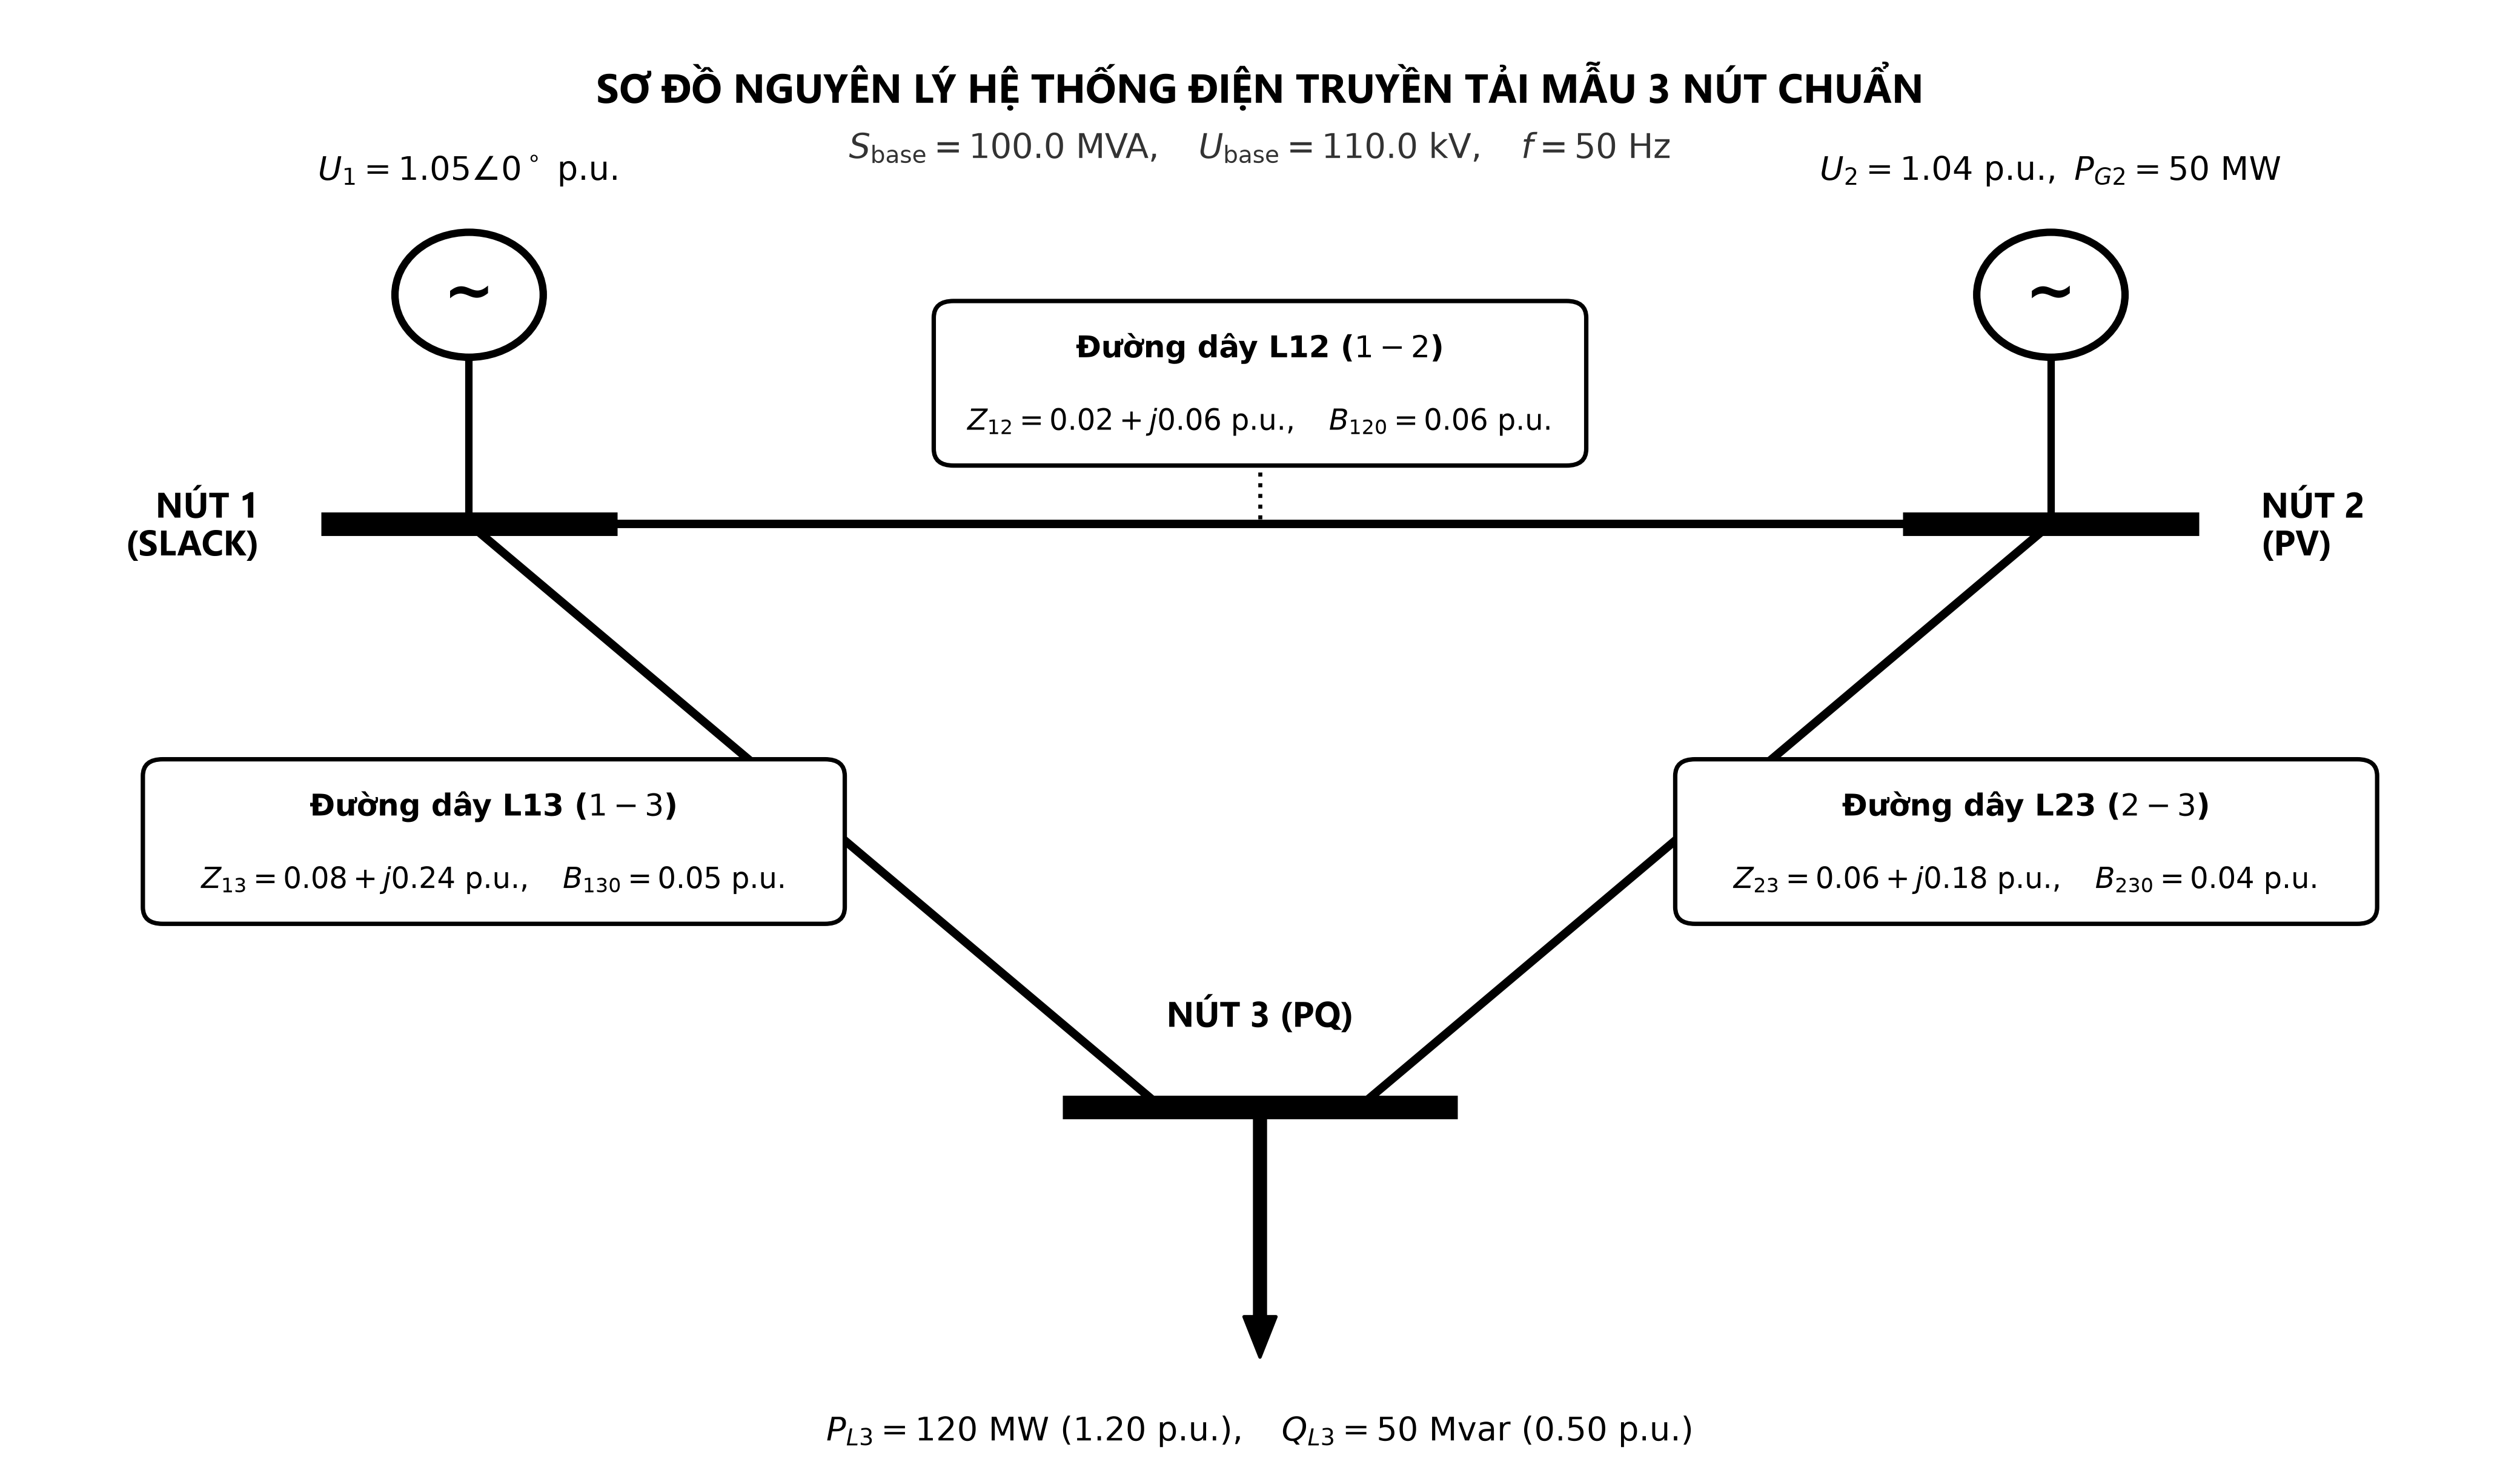
\includegraphics[width=0.65\textwidth]{3bus_network_vi.png}
\caption{Equivalent $\pi$ transmission line circuit and benchmark 3-bus network layout.}
\label{fig:pi_model}
\end{figure}

The series branch impedance is:
\begin{equation}
Z_{ij} = R_{ij} + j X_{ij}\text{ (p.u.)}
\end{equation}
The series branch admittance is:
\begin{equation}
y_{ij} = \frac{1}{Z_{ij}} = \frac{R_{ij}}{R_{ij}^2 + X_{ij}^2} - j \frac{X_{ij}}{R_{ij}^2 + X_{ij}^2} = g_{ij} + j b_{ij}\text{ (p.u.)}
\end{equation}
Total line charging susceptance $B_{ij0}$ is equally split between terminal buses:
\begin{equation}
y_{sh,i} = y_{sh,j} = j \frac{B_{ij0}}{2}\text{ (p.u.)}
\end{equation}

\subsection{3. Transformers and Net Injected Power}
Transmission transformers are modeled via series short-circuit impedance $R_T + jX_T$ and off-nominal tap ratios $k = 1:a$. Net injected complex power at bus $i$ is:
\begin{equation}
S_i^{\text{spec}} = P_i^{\text{spec}} + j Q_i^{\text{spec}} = (P_{Gi} - P_{Li}) + j (Q_{Gi} - Q_{Li})
\end{equation}

\section{KCL Node Current Formulation and Bus Admittance Matrix $\mathbf{Y}_{\text{bus}}$}
By Kirchhoff's Current Law (KCL), the net current injected into bus $i$ must equal the sum of currents flowing out into connected branches and shunt elements:
\begin{equation}
\dot{I}_i = \sum_{j=1}^n Y_{ij} \dot{U}_j \quad \forall i = 1, 2, \dots, n
\end{equation}
In compact matrix notation:
\begin{equation}
\mathbf{I}_{\text{bus}} = \mathbf{Y}_{\text{bus}} \mathbf{U}_{\text{bus}}
\end{equation}
where $\mathbf{I}_{\text{bus}} = [\dot{I}_1, \dots, \dot{I}_n]^T$, $\mathbf{U}_{\text{bus}} = [\dot{U}_1, \dots, \dot{U}_n]^T$, and $\mathbf{Y}_{\text{bus}}$ is the $n \times n$ bus admittance matrix.

\noindent The relationship between complex power and bus current is:
\begin{equation}
S_i = P_i + jQ_i = \dot{U}_i \dot{I}_i^* \implies \dot{I}_i = \frac{S_i^*}{\dot{U}_i^*} = \frac{P_i - jQ_i}{\dot{U}_i^*}
\end{equation}

\noindent Rules for assembling elements of $\mathbf{Y}_{\text{bus}}$:
\begin{itemize}
    \item \textbf{Off-Diagonal Elements ($i \ne j$):} Equal to the negative of the series admittance directly connecting bus $i$ and bus $j$:
    \begin{equation}
    Y_{ij} = Y_{ji} = - y_{ij} = - (g_{ij} + j b_{ij})\text{ (p.u.)}
    \end{equation}
    If no direct connection exists, $Y_{ij} = 0$.
    \item \textbf{Diagonal Elements ($i = j$):} Equal to the sum of all branch series admittances connected to bus $i$, plus total line charging admittances and local shunt elements:
    \begin{equation}
    Y_{ii} = \sum_{j \in \Omega_i} y_{ij} + \sum_{j \in \Omega_i} j \frac{B_{ij0}}{2} + y_{\text{shunt}, i}\text{ (p.u.)}
    \end{equation}
    where $\Omega_i$ is the set of all buses directly connected to bus $i$.
\end{itemize}

\section{Bus Classification and Boundary Conditions (SLACK, PV, PQ)}
Every bus $i$ is characterized by 4 variables: active power $P_i$, reactive power $Q_i$, voltage magnitude $U_i$, and phase angle $\delta_i$. Because only two power balance equations can be formulated per bus, two variables must be specified as inputs while the remaining two are unknowns. Buses are strictly classified into 3 physical categories (Table~\ref{tab:bus_classification}):

\begin{table}[H]
\centering
\caption{Rigorous bus classification and distinction between Specified Inputs and Unknowns.}
\label{tab:bus_classification}
\begin{tabularx}{\textwidth}{lXX}
\toprule
\textbf{Bus Type} & \textbf{SPECIFIED INPUTS (Given)} & \textbf{UNKNOWN STATE VARIABLES (To Solve)} \\
\midrule
\textbf{SLACK} (Swing Bus) & 
- Voltage magnitude $U_i$ ($1.05\text{ p.u.}$) \newline
- Phase angle $\delta_i = 0^\circ$ (Reference) & 
- Active power generation $P_{Gi}$ (Unknown) \newline
- Reactive power generation $Q_{Gi}$ (Unknown) \\
\midrule
\textbf{PV} (Voltage-Controlled) & 
- Active power generation $P_{Gi}$ \newline
- Specified voltage magnitude $U_i$ & 
- Phase angle $\delta_i$ (Unknown state) \newline
- Reactive power generation $Q_{Gi}$ (Unknown) \\
\midrule
\textbf{PQ} (Load Bus) & 
- Active power demand $P_{Li}$ \newline
- Reactive power demand $Q_{Li}$ & 
- Voltage magnitude $U_i$ (Unknown state) \newline
- Phase angle $\delta_i$ (Unknown state) \\
\bottomrule
\end{tabularx}
\end{table}

\noindent \textbf{Core Engineering Principles:}
\begin{itemize}
    \item At the \textbf{SLACK} bus, $P_{G1}$ and $Q_{G1}$ are dependent unknowns responsible for balancing total network transmission losses; they cannot be arbitrarily initialized to zero.
    \item At \textbf{PV} buses, prime mover governors maintain constant active generation $P_{Gi}$ and automatic voltage regulators (AVR) maintain terminal voltage $U_i$. Voltage angle $\delta_i$ and reactive generation $Q_{Gi}$ are unknown variables.
    \item At \textbf{PQ} buses, both $U_i$ and $\delta_i$ are completely unknown state variables. Solvers employ initial flat start assumptions ($U_i^{(0)} = 1.0\text{ p.u.}, \delta_i^{(0)} = 0^\circ$).
\end{itemize}

\section{Load Modeling Under Voltage Variations (PQ vs. ZIP Models)}
A critical aspect of power flow theory is how aggregate loads behave when bus voltage $U$ varies:

\subsection{1. Constant Power Load Model (PQ Model)}
In standard power flow studies, loads are assumed to consume constant power independent of voltage:
\begin{equation}
P_L(U) = P_{L0} = \text{const}, \qquad Q_L(U) = Q_{L0} = \text{const}
\end{equation}
As terminal voltage $U$ drops, the load current $\dot{I}_L = (P_{L0} - jQ_{L0})/\dot{U}^*$ increases inversely ($I \propto 1/U$). Higher current flowing through line impedances produces greater voltage drops $\Delta U = I \cdot Z$, accelerating voltage degradation toward static voltage collapse.

\subsection{2. Voltage-Dependent ZIP Polynomial Load Model}
In practical power networks, composite substation loads exhibit nonlinear voltage dependence modeled via the polynomial ZIP formulation:
\begin{align}
P_L(U) &= P_{L0} \left[ a_1 \left( \frac{U}{U_0} \right)^2 + a_2 \left( \frac{U}{U_0} \right) + a_3 \right] \\
Q_L(U) &= Q_{L0} \left[ b_1 \left( \frac{U}{U_0} \right)^2 + b_2 \left( \frac{U}{U_0} \right) + b_3 \right]
\end{align}
subject to normalization constraints:
\begin{equation}
a_1 + a_2 + a_3 = 1, \qquad b_1 + b_2 + b_3 = 1
\end{equation}
where $U_0$ is nominal voltage and $P_{L0}, Q_{L0}$ denote consumption at nominal voltage. Physical interpretation of each component:
\begin{enumerate}
    \item \textbf{Z Component (Constant Impedance - Quadratic):} Coefficients $a_1, b_1$. Power varies quadratically ($P \propto U^2$), current varies linearly ($I \propto U$). Represents resistive heaters, incandescent lighting, and uncontrolled loads. When voltage drops, power consumption decreases automatically, mitigating grid stress.
    \item \textbf{I Component (Constant Current - Linear):} Coefficients $a_2, b_2$. Power varies linearly ($P \propto U$), current remains constant ($I = \text{const}$). Represents discharge lighting, uncontrolled rectifiers, and partially loaded induction motors.
    \item \textbf{P Component (Constant Power - Independent):} Coefficients $a_3, b_3$. Power is voltage-invariant ($P = \text{const}$), current varies inversely ($I \propto 1/U$). Represents speed-controlled motor drives and power electronics loads.
\end{enumerate}

\section{Nonlinear Algebraic Power Flow Equations}

\subsection{1. Mathematical Formulation}
Substituting KCL nodal currents into complex power equations, expressing voltages in polar coordinates $\dot{U}_i = U_i e^{j\delta_i}$ and admittances in rectangular form $Y_{ij} = G_{ij} + jB_{ij}$:
\begin{align}
P_i + jQ_i &= \dot{U}_i \left( \sum_{j=1}^n Y_{ij} \dot{U}_j \right)^* = U_i e^{j\delta_i} \sum_{j=1}^n (G_{ij} - jB_{ij}) U_j e^{-j\delta_j} \nonumber \\
&= \sum_{j=1}^n U_i U_j (G_{ij} - jB_{ij}) \left[ \cos(\delta_i - \delta_j) + j \sin(\delta_i - \delta_j) \right]
\end{align}
Separating real and imaginary parts yields the classical nonlinear polar power balance equations:
\begin{align}
P_i(\boldsymbol{\delta}, \mathbf{U}) &= U_i^2 G_{ii} + \sum_{j \ne i} U_i U_j \left[ G_{ij} \cos(\delta_i - \delta_j) + B_{ij} \sin(\delta_i - \delta_j) \right] \label{eq:p_polar} \\
Q_i(\boldsymbol{\delta}, \mathbf{U}) &= -\, U_i^2 B_{ii} + \sum_{j \ne i} U_i U_j \left[ G_{ij} \sin(\delta_i - \delta_j) - B_{ij} \cos(\delta_i - \delta_j) \right] \label{eq:q_polar}
\end{align}

\subsection{2. Power Mismatch Equations}
At buses with specified net injections, mismatches between specified and calculated powers must vanish:
\begin{align}
\Delta P_i(\boldsymbol{\delta}, \mathbf{U}) &= P_i^{\text{spec}} - P_i(\boldsymbol{\delta}, \mathbf{U}) = 0 \quad \forall i \in \{2, 3, \dots, n\} \\
\Delta Q_i(\boldsymbol{\delta}, \mathbf{U}) &= Q_i^{\text{spec}} - Q_i(\boldsymbol{\delta}, \mathbf{U}) = 0 \quad \forall i \in \{\text{PQ buses}\}
\end{align}

\subsection{3. State Variable Unknowns Vector}
For an $n$-bus network with bus 1 as Slack, $N_{PV}$ PV buses, and $N_{PQ}$ PQ buses ($n = 1 + N_{PV} + N_{PQ}$), the vector of unknown state variables is:
\begin{equation}
\mathbf{x} = 
\begin{bmatrix}
\delta_2 \\
\vdots \\
\delta_n \\
U_{m+1} \\
\vdots \\
U_n
\end{bmatrix}
\in \mathbb{R}^{(2n - 2 - N_{PV})}
\end{equation}

\subsection{4. Converged Solution Vector}
The solution is the converged state vector $\mathbf{x}^* = [\boldsymbol{\delta}^*, \mathbf{U}^*]$ satisfying:
\begin{equation}
\Vert \Delta \mathbf{f}(\mathbf{x}^*) \Vert_\infty = \max \left( \max_{i} |\Delta P_i(\mathbf{x}^*)|, \max_{i} |\Delta Q_i(\mathbf{x}^*)| \right) \le \varepsilon = 10^{-10}\text{ p.u.}
\end{equation}

\subsection{5. Operational Output Quantities}
Once $\mathbf{x}^*$ is obtained, all operational parameters are calculated directly:
\begin{enumerate}
    \item Slack bus generation: $P_{G1} = P_1(\mathbf{x}^*) + P_{L1}$, $Q_{G1} = Q_1(\mathbf{x}^*) + Q_{L1}$.
    \item PV bus reactive generation: $Q_{Gi} = Q_i(\mathbf{x}^*) + Q_{Li}$ ($i \in \text{PV}$).
    \item Complex branch flows from bus $i$ to bus $j$:
    \begin{equation}
    S_{ij} = P_{ij} + jQ_{ij} = \dot{U}_i \left[ (\dot{U}_i - \dot{U}_j) y_{ij} + \dot{U}_i \left( j \frac{B_{ij0}}{2} \right) \right]^*
    \end{equation}
    \item Branch power losses $\Delta S_{ij} = S_{ij} + S_{ji}$ and total active transmission loss $\Delta P_{\text{loss}} = \sum P_{Gi} - \sum P_{Li}$.
\end{enumerate}

% ==================== CHAPTER 3 ====================
\chapter{The Newton--Raphson Algorithm and Solver Software Tool}

\section{Analytical Foundations of Polar Newton--Raphson Formulation}
Because the power flow equations are transcendental, closed-form solutions do not exist. The Newton--Raphson method applies a first-order Taylor expansion around the current operating point $\mathbf{x}^{(m)}$:
\begin{equation}
\mathbf{f}(\mathbf{x}^{(m)} + \Delta \mathbf{x}^{(m)}) \approx \mathbf{f}(\mathbf{x}^{(m)}) + \left[ \frac{\partial \mathbf{f}}{\partial \mathbf{x}} \right]^{(m)} \Delta \mathbf{x}^{(m)} = \mathbf{0}
\end{equation}
Neglecting higher-order terms, the nonlinear system is linearized into:
\begin{equation}
\begin{bmatrix}
\Delta \mathbf{P}^{(m)} \\[4pt]
\Delta \mathbf{Q}^{(m)}
\end{bmatrix}
=
\begin{bmatrix}
\mathbf{H}^{(m)} & \mathbf{N}^{(m)} \\[4pt]
\mathbf{M}^{(m)} & \mathbf{L}^{(m)}
\end{bmatrix}
\begin{bmatrix}
\Delta \boldsymbol{\delta}^{(m)} \\[4pt]
\Delta \mathbf{U}^{(m)} / \mathbf{U}^{(m)}
\end{bmatrix}
= \mathbf{J}^{(m)} \Delta \mathbf{x}^{(m)}
\end{equation}
where $\mathbf{J}^{(m)}$ is the $(2n - 2 - N_{PV}) \times (2n - 2 - N_{PV})$ Jacobian matrix.

\section{Eight Closed-Form Analytical Jacobian Formulas}
To guarantee exact mathematical precision without finite-difference truncation error, 8 analytical partial derivative expressions are derived directly (Table~\ref{tab:jacobian_formulas}):

\begin{table}[H]
\centering
\caption{Exact closed-form analytical formulas for the 8 sub-blocks of Jacobian $\mathbf{J}$.}
\label{tab:jacobian_formulas}
\resizebox{\textwidth}{!}{\begin{tabular}{ccl}
\toprule
\textbf{Block} & \textbf{Position} & \textbf{Analytical Partial Derivative Expression} \\
\midrule
$\mathbf{H}$ & Off-Diagonal ($j \ne i$) & $H_{ij} = \frac{\partial P_i}{\partial \delta_j} = U_i U_j \left[ G_{ij} \sin(\delta_i - \delta_j) - B_{ij} \cos(\delta_i - \delta_j) \right]$ \\
$\mathbf{H}$ & Diagonal ($j = i$) & $H_{ii} = \frac{\partial P_i}{\partial \delta_i} = -\, Q_i - U_i^2 B_{ii}$ \\
\midrule
$\mathbf{N}$ & Off-Diagonal ($j \ne i$) & $N_{ij} = U_j \frac{\partial P_i}{\partial U_j} = U_i U_j \left[ G_{ij} \cos(\delta_i - \delta_j) + B_{ij} \sin(\delta_i - \delta_j) \right]$ \\
$\mathbf{N}$ & Diagonal ($j = i$) & $N_{ii} = U_i \frac{\partial P_i}{\partial U_i} = P_i + U_i^2 G_{ii}$ \\
\midrule
$\mathbf{M}$ & Off-Diagonal ($j \ne i$) & $M_{ij} = \frac{\partial Q_i}{\partial \delta_j} = -\, N_{ij} = -\, U_i U_j \left[ G_{ij} \cos(\delta_i - \delta_j) + B_{ij} \sin(\delta_i - \delta_j) \right]$ \\
$\mathbf{M}$ & Diagonal ($j = i$) & $M_{ii} = \frac{\partial Q_i}{\partial \delta_i} = P_i - U_i^2 G_{ii}$ \\
\midrule
$\mathbf{L}$ & Off-Diagonal ($j \ne i$) & $L_{ij} = U_j \frac{\partial Q_i}{\partial U_j} = H_{ij} = U_i U_j \left[ G_{ij} \sin(\delta_i - \delta_j) - B_{ij} \cos(\delta_i - \delta_j) \right]$ \\
$\mathbf{L}$ & Diagonal ($j = i$) & $L_{ii} = U_i \frac{\partial Q_i}{\partial U_i} = Q_i - U_i^2 B_{ii}$ \\
\bottomrule
\end{tabular}}
\end{table}

\section{Step-by-Step Algorithmic Procedure and IEEE Flowchart}
The iterative procedure follows 6 sequential stages:
\begin{enumerate}
    \item \textbf{Stage 1 (Initialization):} Read network data, build $\mathbf{Y}_{\text{bus}}$. Initialize flat start: $m = 0, \delta_i^{(0)} = 0^\circ$ for all buses, $U_i^{(0)} = 1.0\text{ p.u.}$ for PQ buses.
    \item \textbf{Stage 2 (Nodal Power Calculation):} Evaluate $P_i^{(m)}, Q_i^{(m)}$ via polar power equations.
    \item \textbf{Stage 3 (Mismatch Evaluation):} Compute $\Delta P_i^{(m)} = P_i^{\text{spec}} - P_i^{(m)}$ and $\Delta Q_i^{(m)} = Q_i^{\text{spec}} - Q_i^{(m)}$.
    \item \textbf{Stage 4 (Convergence Assessment):} Check $\Vert \Delta \mathbf{f}^{(m)} \Vert_\infty \le \varepsilon = 10^{-10}\text{ p.u.}$ If satisfied, proceed to Stage 6.
    \item \textbf{Stage 5 (Jacobian Solution \& State Update):} Evaluate $\mathbf{J}^{(m)}$, solve $\Delta \mathbf{x}^{(m)} = [\mathbf{J}^{(m)}]^{-1}\Delta \mathbf{f}^{(m)}$, update state variables $\delta_i^{(m+1)} = \delta_i^{(m)} + \Delta \delta_i^{(m)}$, $U_i^{(m+1)} = U_i^{(m)} + \Delta U_i^{(m)}$, increment $m \leftarrow m+1$, and return to Stage 2.
    \item \textbf{Stage 6 (Post-Convergence Solution):} Calculate slack bus generation, PV bus reactive power, branch power flows $S_{ij}$, and system losses.
\end{enumerate}

\begin{figure}[H]
\centering
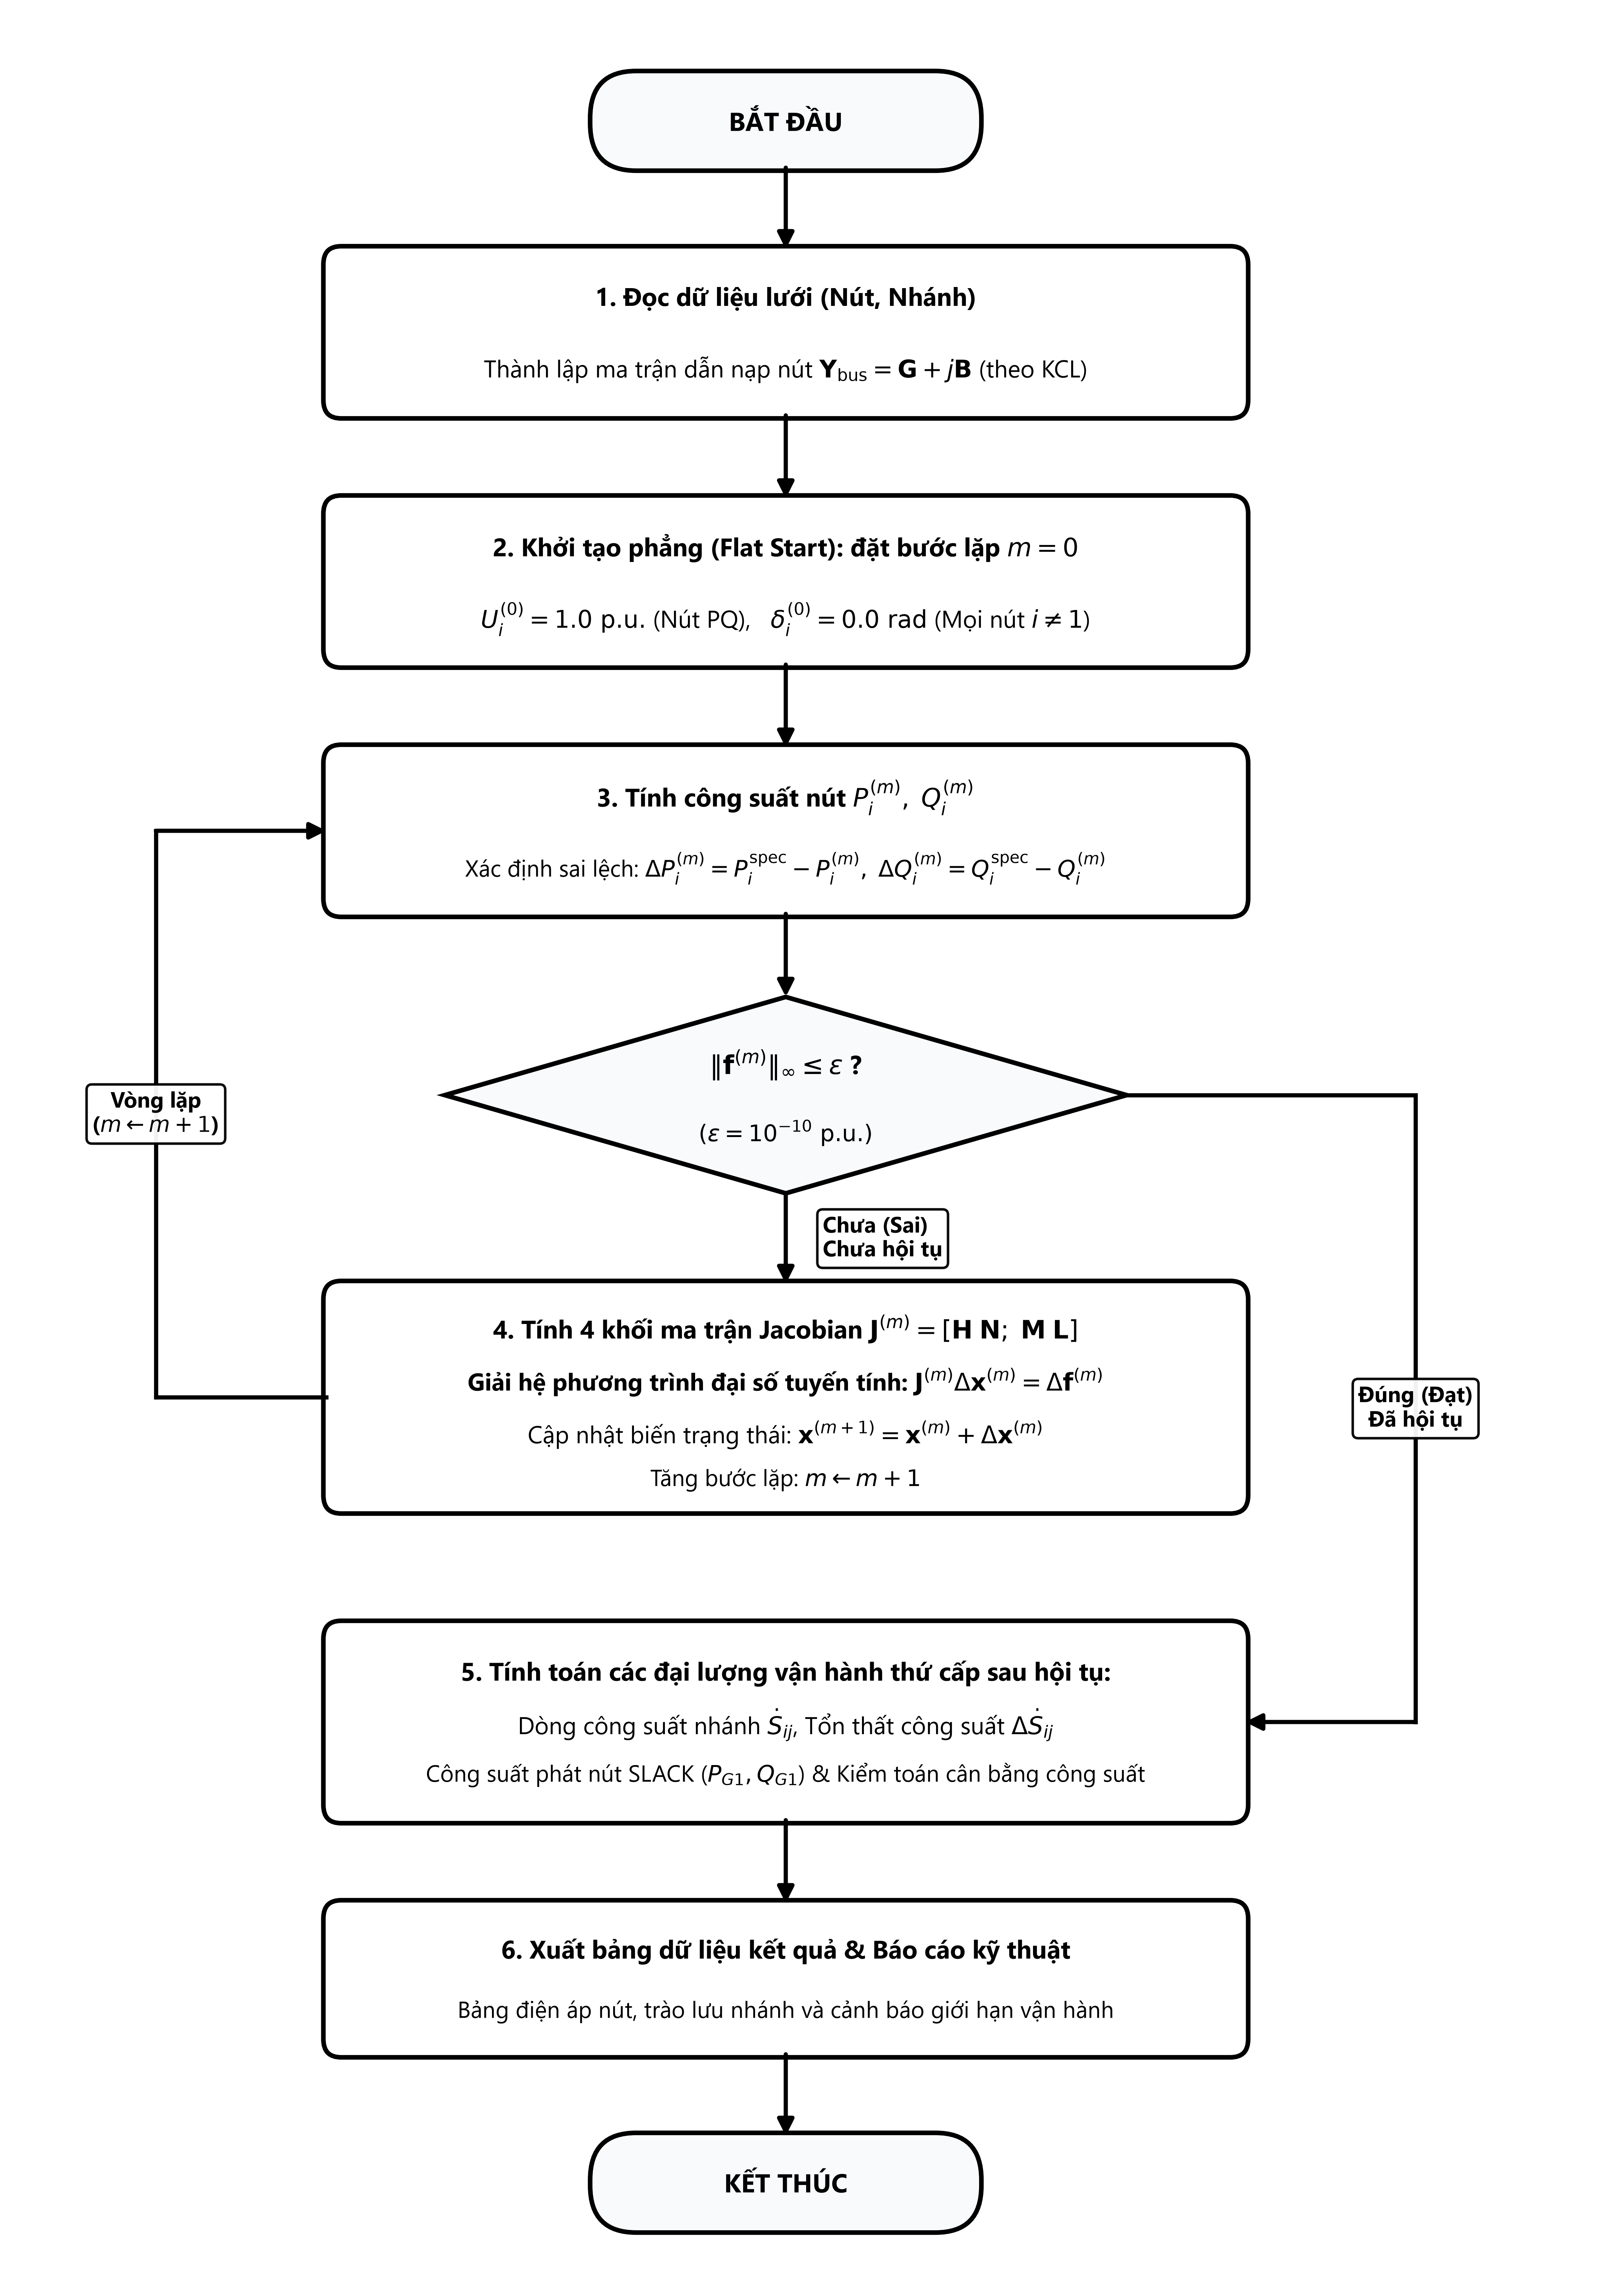
\includegraphics[width=0.70\textwidth]{algorithm_vi.png}
\caption{Newton--Raphson polar power flow algorithm flowchart (IEEE Standard format).}
\label{fig:algorithm_flowchart}
\end{figure}

\section{Introduction to the Software Tool (PowerFlow Desktop Application)}
To support hand-calculation verification and multi-scenario studies, this project utilizes the existing \textbf{PowerFlow (Desktop GUI)} application:

\begin{figure}[H]
\centering
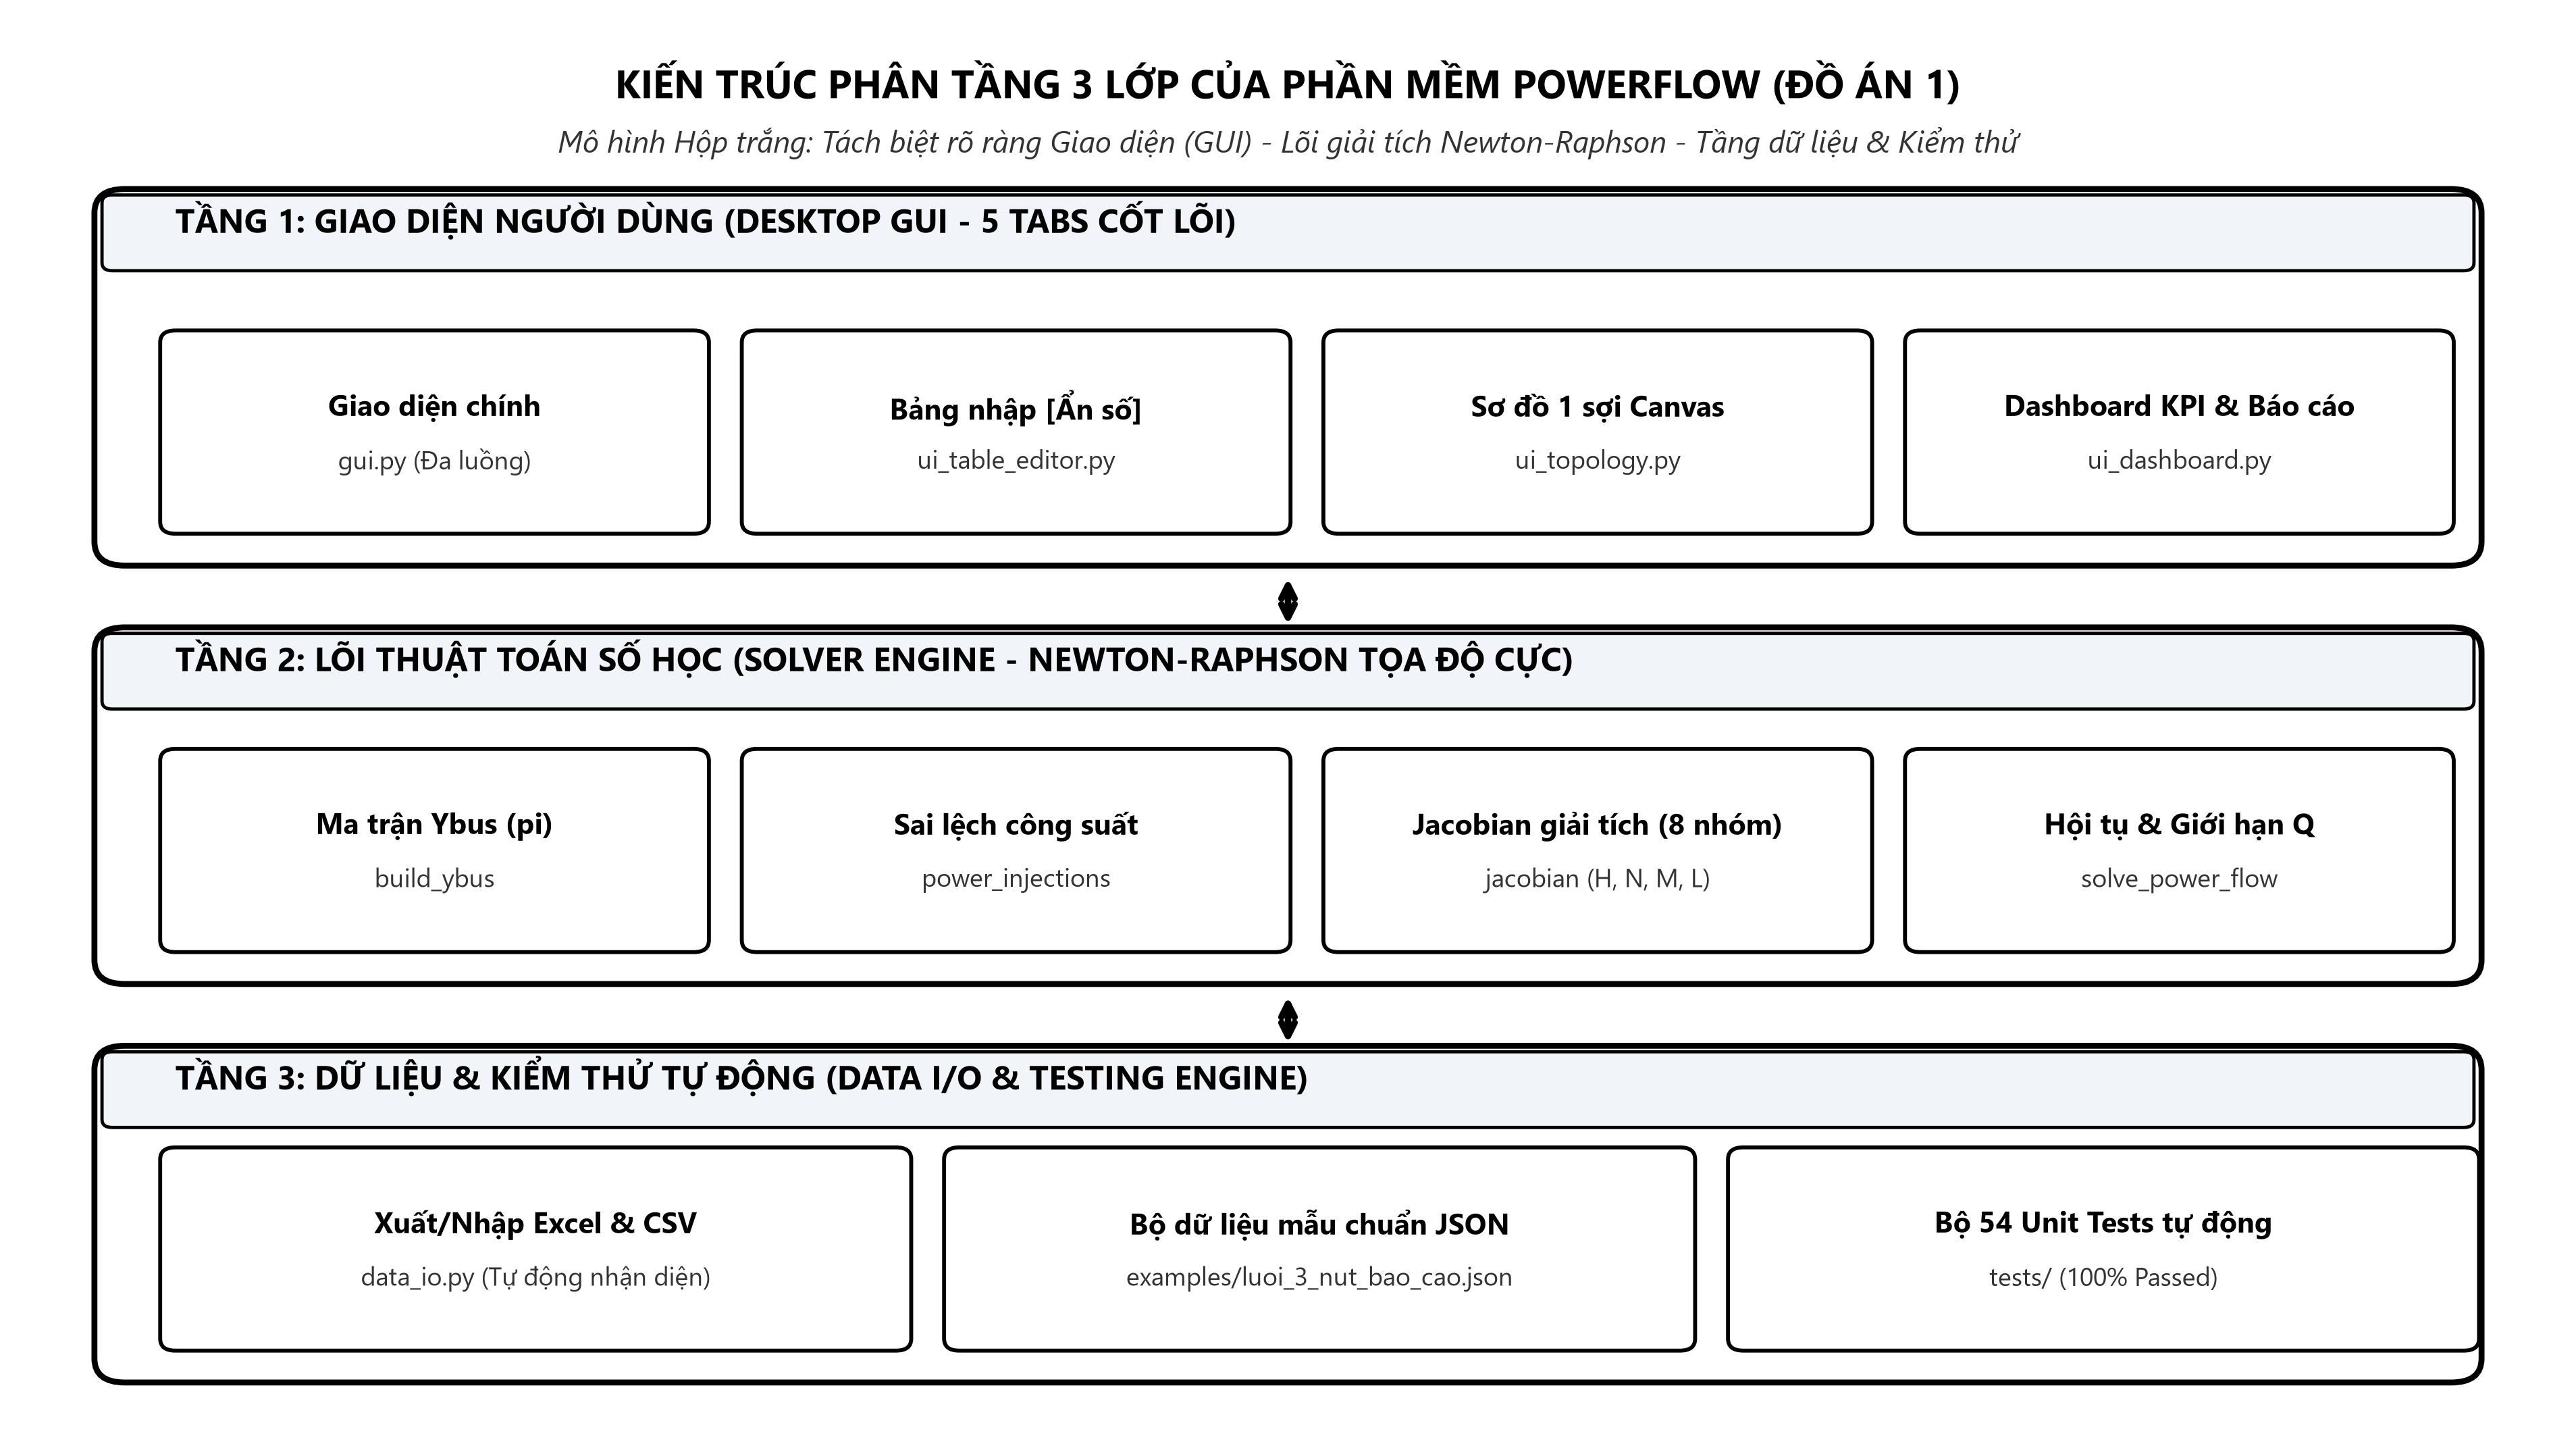
\includegraphics[width=0.92\textwidth]{powerflow_app_architecture.png}
\caption{Three-tier software architecture of the PowerFlow benchmarking tool.}
\label{fig:app_arch}
\end{figure}

\begin{itemize}
    \item \textbf{Tool Positioning:} An existing standalone Python/Tkinter application executing pure polar Newton--Raphson iterations with double-precision floating-point arithmetic.
    \item \textbf{Data Pipeline:} Input network data $\to$ Automated $\mathbf{Y}_{\text{bus}}$ assembly $\to$ Newton--Raphson solver $\to$ Comprehensive output reporting (Voltages, Flows, Losses, Energy Balance).
    \item \textbf{Pedagogical Smart Table Design (Figure~\ref{fig:smart_table}):} Explicitly separates specified inputs from unknown state variables, locking unknown cells and labeling them \textbf{\texttt{[Unknown]}} to avoid erroneous zero initialization.
\end{itemize}

\begin{figure}[H]
\centering
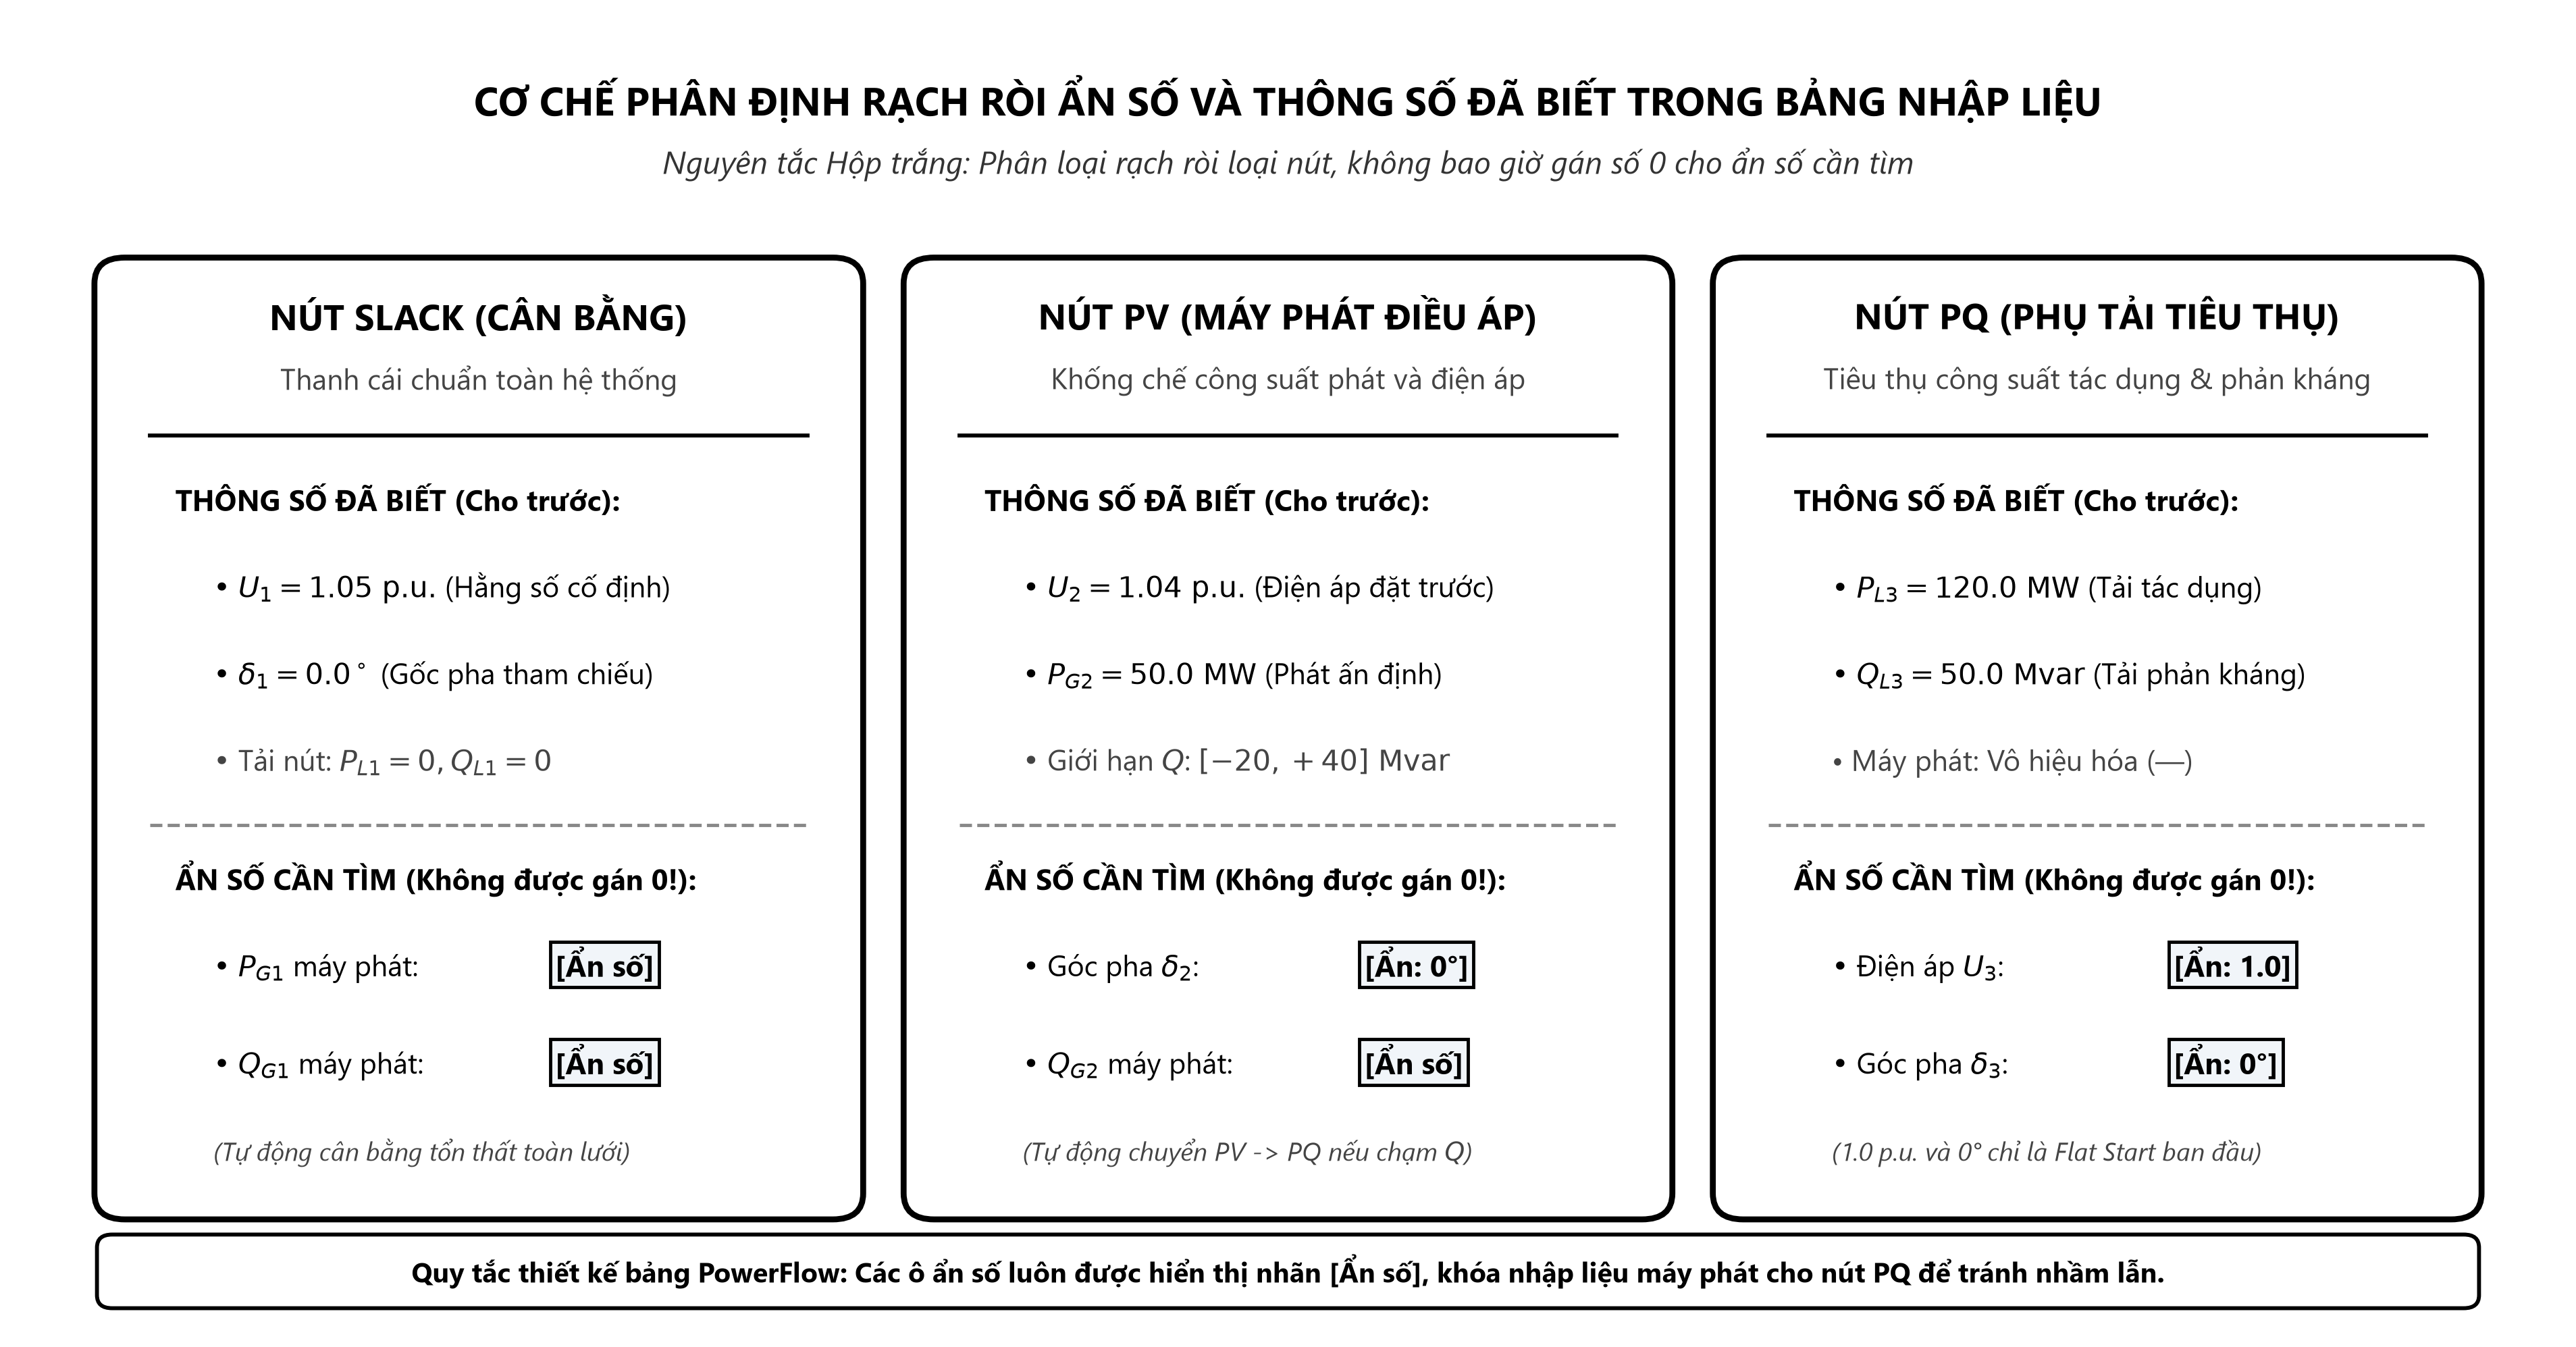
\includegraphics[width=0.95\textwidth]{powerflow_smart_table.png}
\caption{Smart table editor distinguishing specified inputs from unknown variables.}
\label{fig:smart_table}
\end{figure}

\subsection{Actual Graphical User Interface and Interactive Features}
Actual screenshots captured directly from the live desktop \textbf{PowerFlow} application solving the 3-bus transmission system are presented in Figure~\ref{fig:app_gui_dashboard} and Figure~\ref{fig:app_gui_topology}:

\begin{figure}[H]
\centering
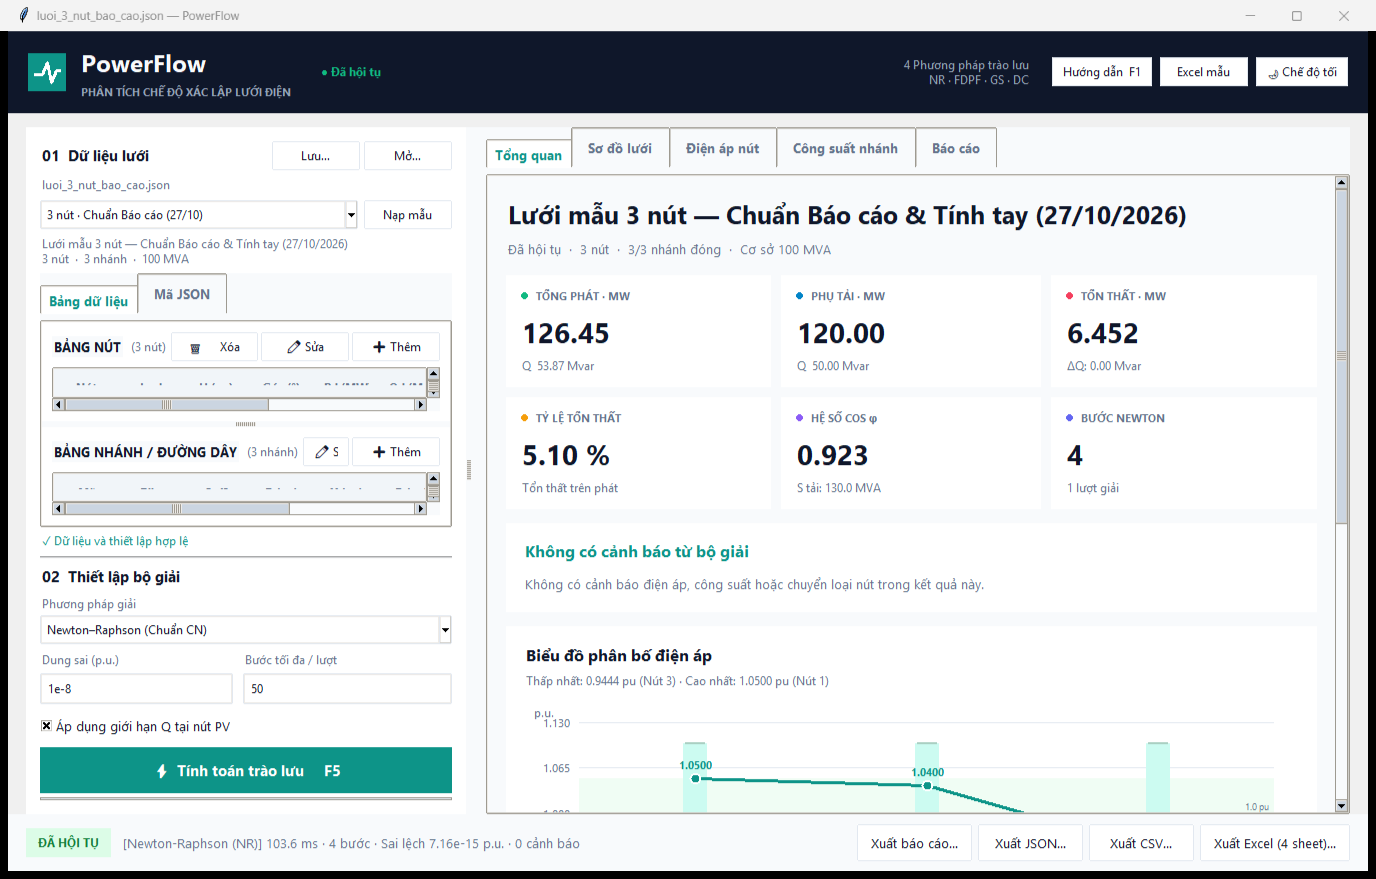
\includegraphics[width=0.98\textwidth]{app_screenshot_dashboard.png}
\caption{Live executive dashboard interface of the PowerFlow application solving the benchmark 3-bus system (Quadratic convergence reached in 4 iterations, generation and loss KPIs, and nodal voltage distribution profile).}
\label{fig:app_gui_dashboard}
\end{figure}

\begin{figure}[H]
\centering
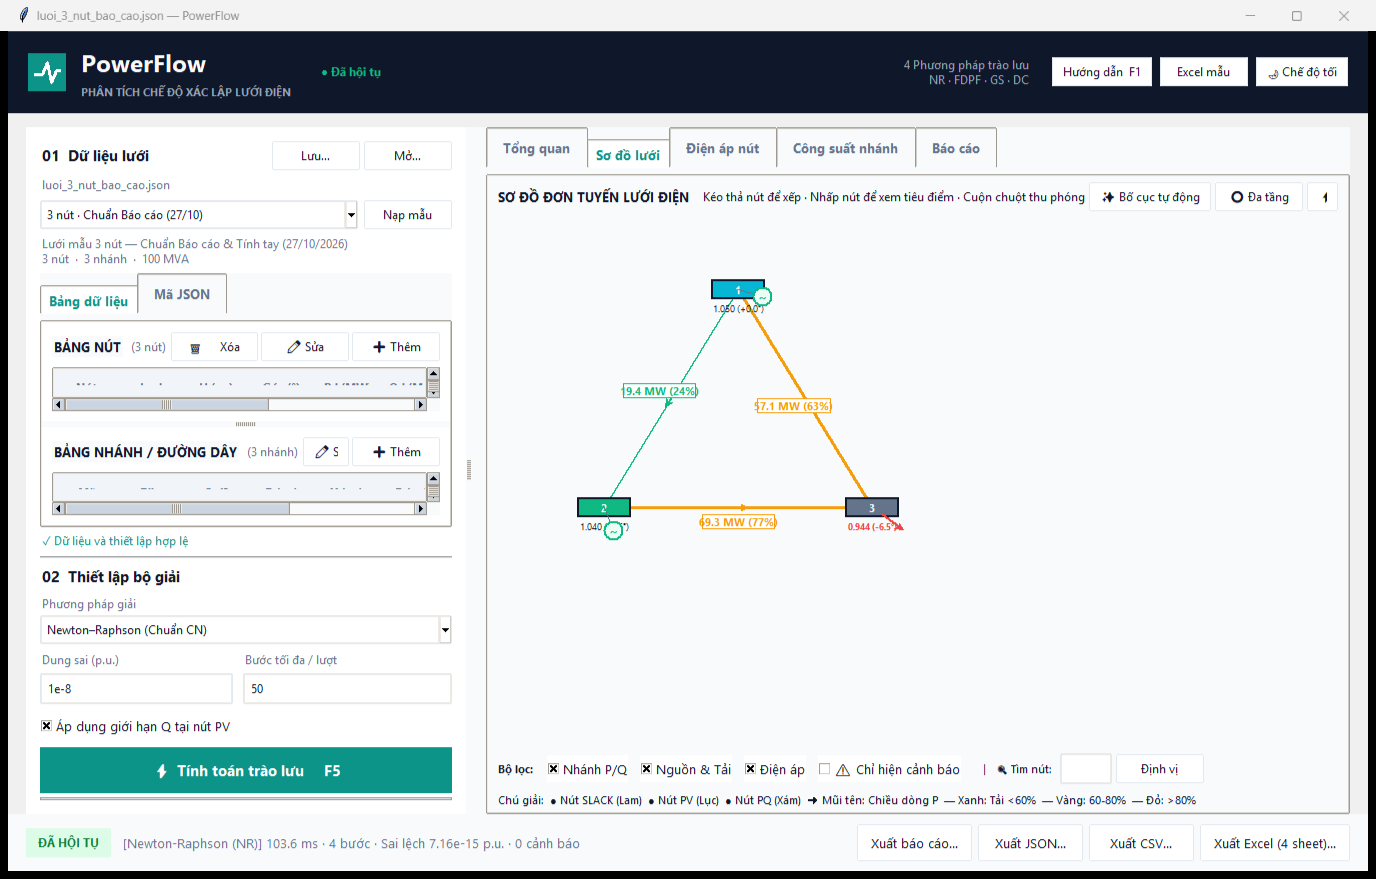
\includegraphics[width=0.98\textwidth]{app_screenshot_topology.png}
\caption{Interactive single-line diagram canvas of the PowerFlow tool (Visualizing real-time active/reactive branch power flows and transmission line loading percentages).}
\label{fig:app_gui_topology}
\end{figure}

% ==================== CHAPTER 4 ====================
\chapter{Step-by-Step Hand Calculation and Software Benchmarking}

\section{Input Specifications of the Standard 3-Bus Benchmark Network}
The standard 3-bus transmission network ($S_{\text{base}} = 100.0\text{ MVA}$, $U_{\text{base}} = 110\text{ kV}$) is specified as follows:
\begin{itemize}
    \item \textbf{Bus 1 (SLACK):} Swing bus, $U_1 = 1.05\text{ p.u.}$, $\delta_1 = 0.0^\circ = 0.0\text{ rad}$.
    \item \textbf{Bus 2 (PV):} Generator bus, $P_{G2} = 50.0\text{ MW} = 0.50\text{ p.u.}$, $U_2 = 1.04\text{ p.u.}$.
    \item \textbf{Bus 3 (PQ):} Concentrated industrial load: \newline
    $P_{L3} = 120.0\text{ MW} = 1.20\text{ p.u.}$, $Q_{L3} = 50.0\text{ Mvar} = 0.50\text{ p.u.}$.
\end{itemize}

\begin{table}[H]
\centering
\caption{Nodal specifications of the 3-bus benchmark transmission system.}
\label{tab:3bus_nodal_data}
\resizebox{\textwidth}{!}{\begin{tabular}{ccccccc}
\toprule
\textbf{Bus} & \textbf{Type} & $U_i\text{ (p.u.)}$ & $\delta_i\text{ (rad)}$ & $P_{Gi}\text{ (p.u.)}$ & $P_{Li}\text{ (p.u.)}$ & $Q_{Li}\text{ (p.u.)}$ \\
\midrule
1 & SLACK & $1.05$ & $0.0000$ & [To Solve] & $0.00$ & $0.00$ \\
2 & PV & $1.04$ & [To Solve] & $0.50$ ($50\text{ MW}$) & $0.00$ & $0.00$ \\
3 & PQ & [To Solve] & [To Solve] & $0.00$ & $1.20$ ($120\text{ MW}$) & $0.50$ ($50\text{ Mvar}$) \\
\bottomrule
\end{tabular}}
\end{table}

\begin{table}[H]
\centering
\caption{Branch parameters of equivalent $\pi$ transmission lines ($S_{\text{base}} = 100.0\text{ MVA}$).}
\label{tab:3bus_branch_data}
\resizebox{\textwidth}{!}{\begin{tabular}{ccccc}
\toprule
\textbf{Branch} & \textbf{From -- To} & Resistance $R_{ij}\text{ (p.u.)}$ & Reactance $X_{ij}\text{ (p.u.)}$ & Charging Susceptance $B_{ij0}\text{ (p.u.)}$ \\
\midrule
1 & $1 - 2$ & $0.02$ & $0.06$ & $0.06$ \\
2 & $1 - 3$ & $0.08$ & $0.24$ & $0.05$ \\
3 & $2 - 3$ & $0.06$ & $0.18$ & $0.04$ \\
\bottomrule
\end{tabular}}
\end{table}

\noindent $\blacktriangleright$ \textbf{Specified Net Injections ($P_i^{\text{spec}} = P_{Gi} - P_{Li}$, $Q_i^{\text{spec}} = Q_{Gi} - Q_{Li}$):}
\begin{align}
P_2^{\text{spec}} &= 0.50 - 0.00 = \mathbf{0.500000\text{ p.u.}} \\
P_3^{\text{spec}} &= 0.00 - 1.20 = \mathbf{-1.200000\text{ p.u.}} \\
Q_3^{\text{spec}} &= 0.00 - 0.50 = \mathbf{-0.500000\text{ p.u.}}
\end{align}

\section{Detailed Step-by-Step Hand Calculations (Iteration 1)}

\subsection{Step 1: Branch Admittances and $\mathbf{Y}_{\text{bus}}$ Matrix}
Evaluating branch series admittances:
\begin{align}
y_{12} &= \frac{1}{0.02 + j0.06} = \frac{0.02}{0.0040} - j\frac{0.06}{0.0040} = \mathbf{5.000000 - j15.000000\text{ p.u.}} \\
y_{13} &= \frac{1}{0.08 + j0.24} = \frac{0.08}{0.0640} - j\frac{0.24}{0.0640} = \mathbf{1.250000 - j3.750000\text{ p.u.}} \\
y_{23} &= \frac{1}{0.06 + j0.18} = \frac{0.06}{0.0360} - j\frac{0.18}{0.0360} = \mathbf{1.666667 - j5.000000\text{ p.u.}}
\end{align}
Evaluating diagonal elements including branch charging susceptances:
\begin{align}
Y_{11} &= y_{12} + y_{13} + j(0.06/2 + 0.05/2) = \mathbf{6.250000 - j18.695000\text{ p.u.}} \\
Y_{22} &= y_{12} + y_{23} + j(0.06/2 + 0.04/2) = \mathbf{6.666667 - j19.950000\text{ p.u.}} \\
Y_{33} &= y_{13} + y_{23} + j(0.05/2 + 0.04/2) = \mathbf{2.916667 - j8.705000\text{ p.u.}}
\end{align}
Off-diagonal elements:
\begin{align}
Y_{12} = Y_{21} &= -\, y_{12} = \mathbf{-5.000000 + j15.000000\text{ p.u.}} \\
Y_{13} = Y_{31} &= -\, y_{13} = \mathbf{-1.250000 + j3.750000\text{ p.u.}} \\
Y_{23} = Y_{32} &= -\, y_{23} = \mathbf{-1.666667 + j5.000000\text{ p.u.}}
\end{align}
The assembled bus admittance matrix:
\begin{equation}
\resizebox{\linewidth}{!}{$
\mathbf{Y}_{\text{bus}} = 
\begin{bmatrix}
6.250000 - j18.695000 & -5.000000 + j15.000000 & -1.250000 + j3.750000 \\[4pt]
-5.000000 + j15.000000 & 6.666667 - j19.950000 & -1.666667 + j5.000000 \\[4pt]
-1.250000 + j3.750000 & -1.666667 + j5.000000 & 2.916667 - j8.705000
\end{bmatrix}\text{ (p.u.)}
$}
\end{equation}

\subsection{Step 2: Flat Start Initialization and Power Mismatches}
Flat start initialization at iteration $m = 0$:
\begin{align}
\delta_1^{(0)} &= 0.0\text{ rad}, \quad \delta_2^{(0)} = 0.0\text{ rad}, \quad \delta_3^{(0)} = 0.0\text{ rad} \\
U_1 &= 1.05\text{ p.u.}, \quad U_2 = 1.04\text{ p.u.}, \quad U_3^{(0)} = 1.00\text{ p.u.}
\end{align}
Since initial angles are zero, $\cos(\delta_i - \delta_j) = 1$ and $\sin(\delta_i - \delta_j) = 0$. Powers evaluated:
\begin{align}
P_2^{(0)} &= (1.04)^2(6.666667) + (1.04)(1.05)(-5.0) + (1.04)(1.0)(-1.666667) = \mathbf{0.017333\text{ p.u.}} \\
P_3^{(0)} &= (1.0)^2(2.916667) + (1.0)(1.05)(-1.25) + (1.0)(1.04)(-1.666667) = \mathbf{-0.129167\text{ p.u.}} \\
Q_3^{(0)} &= -(1.0)^2(-8.705) - (1.0)(1.05)(3.75) - (1.0)(1.04)(5.0) = \mathbf{-0.432500\text{ p.u.}}
\end{align}
Mismatch vector:
\begin{align}
\Delta P_2^{(0)} &= 0.500000 - 0.017333 = \mathbf{0.482667\text{ p.u.}} \\
\Delta P_3^{(0)} &= -1.200000 - (-0.129167) = \mathbf{-1.070833\text{ p.u.}} \\
\Delta Q_3^{(0)} &= -0.500000 - (-0.432500) = \mathbf{-0.067500\text{ p.u.}}
\end{align}
Maximum infinity norm error: $\Vert \Delta \mathbf{f}^{(0)} \Vert_\infty = 1.070833\text{ p.u.} \gg 10^{-10}\text{ p.u.}$

\subsection{Step 3: Evaluation of the 9 Elements of Jacobian $\mathbf{J}^{(0)}$}
Reactive power computed at bus 2 under flat start:
\begin{equation}
Q_2^{(0)} = -(1.04)^2(-19.95) - (1.04)(1.05)(15.0) - (1.04)(1.0)(5.0) = \mathbf{-0.002080\text{ p.u.}}
\end{equation}
Evaluating the 9 Jacobian elements:
\begin{align}
H_{22} &= -(-0.002080) - (1.04)^2 (-19.950000) = \mathbf{21.580000} \\
H_{23} &= -\, (1.04)(1.0)(5.0) = \mathbf{-5.200000} \\
H_{32} &= -\, (1.0)(1.04)(5.0) = \mathbf{-5.200000} \\
H_{33} &= -(-0.432500) - (1.0)^2 (-8.705000) = \mathbf{9.137500} \\
N_{23} &= (1.04)(1.0)(-1.666667) = \mathbf{-1.733333} \\
N_{33} &= -0.129167 + (1.0)^2 (2.916667) = \mathbf{2.787500} \\
M_{32} &= -\, (1.0)(1.04)(-1.666667) = \mathbf{1.733333} \\
M_{33} &= -0.129167 - (1.0)^2 (2.916667) = \mathbf{-3.045833} \\
L_{33} &= -0.432500 - (1.0)^2 (-8.705000) = \mathbf{8.272500}
\end{align}
The linearized matrix equation is:
\begin{equation}
\begin{bmatrix}
21.580000 & -5.200000 & -1.733333 \\
-5.200000 & 9.137500 & 2.787500 \\
1.733333 & -3.045833 & 8.272500
\end{bmatrix}
\begin{bmatrix}
\Delta \delta_2^{(0)} \\[3pt]
\Delta \delta_3^{(0)} \\[3pt]
\Delta U_3^{(0)}
\end{bmatrix}
=
\begin{bmatrix}
0.482667 \\[3pt]
-1.070833 \\[3pt]
-0.067500
\end{bmatrix}
\end{equation}

\subsection{Step 4: Matrix Inversion and State Update}
Determinant $\det(\mathbf{J}^{(0)}) = 1279.799781$. The inverse matrix is:
\begin{equation}
[\mathbf{J}^{(0)}]^{-1} = 
\begin{bmatrix}
0.065670 & 0.037380 & 0.001183 \\
0.037372 & 0.141979 & -0.039984 \\
-0.000021 & 0.044342 & 0.132890
\end{bmatrix}
\end{equation}
Computing the correction vector:
\begin{align}
\Delta \delta_2^{(0)} &= 0.065670(0.482667) + 0.037380(-1.070833) \nonumber \\
&\quad + 0.001183(-0.067500) = \mathbf{-0.007170\text{ rad}} \\
\Delta \delta_3^{(0)} &= 0.037372(0.482667) + 0.141979(-1.070833) \nonumber \\
&\quad - 0.039984(-0.067500) = \mathbf{-0.107200\text{ rad}} \\
\Delta U_3^{(0)} &= -0.000021(0.482667) + 0.044342(-1.070833) \nonumber \\
&\quad + 0.132890(-0.067500) = \mathbf{-0.046127\text{ p.u.}}
\end{align}
Updating state variables for Iteration 1 ($m = 1$):
\begin{align}
\delta_2^{(1)} &= \delta_2^{(0)} + \Delta \delta_2^{(0)} = \mathbf{-0.007170\text{ rad}}\ (-0.410811^\circ) \\
\delta_3^{(1)} &= \delta_3^{(0)} + \Delta \delta_3^{(0)} = \mathbf{-0.107200\text{ rad}}\ (-6.142079^\circ) \\
U_3^{(1)} &= U_3^{(0)} + \Delta U_3^{(0)} = 1.000000 - 0.046127 = \mathbf{0.953873\text{ p.u.}}
\end{align}

\section{1:1 Cross-Validation: Hand Calculations vs. PowerFlow Tool}
All hand-calculated results are rigorously compared against the output generated by the PowerFlow software tool (Table~\ref{tab:cross_validation_iter1}):

\begin{table}[H]
\centering
\caption{Cross-validation comparison at Iteration 1 (Hand Calculations vs. PowerFlow Tool).}
\label{tab:cross_validation_iter1}
\resizebox{\textwidth}{!}{\begin{tabular}{lrrr}
\toprule
\textbf{Validation Quantity} & \textbf{Hand Calculation (Casio)} & \textbf{PowerFlow Tool (Python)} & \textbf{Absolute Deviation} \\
\midrule
Power mismatch $\Delta P_2^{(0)}\text{ (p.u.)}$ & $0.48266667$ & $0.48266667$ & $0.00000000$ \\
Power mismatch $\Delta P_3^{(0)}\text{ (p.u.)}$ & $-1.07083333$ & $-1.07083333$ & $0.00000000$ \\
Power mismatch $\Delta Q_3^{(0)}\text{ (p.u.)}$ & $-0.06750000$ & $-0.06750000$ & $0.00000000$ \\
\midrule
Jacobian element $H_{22}^{(0)}$ & $21.58000000$ & $21.58000000$ & $0.00000000$ \\
Jacobian element $H_{23}^{(0)}$ & $-5.20000000$ & $-5.20000000$ & $0.00000000$ \\
Jacobian element $H_{33}^{(0)}$ & $9.13750000$ & $9.13750000$ & $0.00000000$ \\
Jacobian element $N_{23}^{(0)}$ & $-1.73333333$ & $-1.73333333$ & $0.00000000$ \\
Jacobian element $N_{33}^{(0)}$ & $2.78750000$ & $2.78750000$ & $0.00000000$ \\
Jacobian element $M_{32}^{(0)}$ & $1.73333333$ & $1.73333333$ & $0.00000000$ \\
Jacobian element $M_{33}^{(0)}$ & $-3.04583333$ & $-3.04583333$ & $0.00000000$ \\
Jacobian element $L_{33}^{(0)}$ & $8.27250000$ & $8.27250000$ & $0.00000000$ \\
\midrule
Angle correction $\Delta \delta_2^{(0)}\text{ (rad)}$ & $-0.00716985$ & $-0.00716985$ & $< 10^{-16}$ \\
Angle correction $\Delta \delta_3^{(0)}\text{ (rad)}$ & $-0.10719976$ & $-0.10719976$ & $< 10^{-16}$ \\
Voltage correction $\Delta U_3^{(0)}\text{ (p.u.)}$ & $-0.04612691$ & $-0.04612691$ & $< 10^{-16}$ \\
\midrule
Bus 3 voltage after Iter 1 $U_3^{(1)}\text{ (p.u.)}$ & $0.95387309$ & $0.95387309$ & $< 10^{-16}$ \\
Bus 2 angle after Iter 1 $\delta_2^{(1)}\text{ (deg)}$ & $-0.410802^\circ$ & $-0.410802^\circ$ & $< 10^{-14}$ \\
Bus 3 angle after Iter 1 $\delta_3^{(1)}\text{ (deg)}$ & $-6.142079^\circ$ & $-6.142079^\circ$ & $< 10^{-14}$ \\
\bottomrule
\end{tabular}}
\end{table}

\begin{figure}[H]
\centering
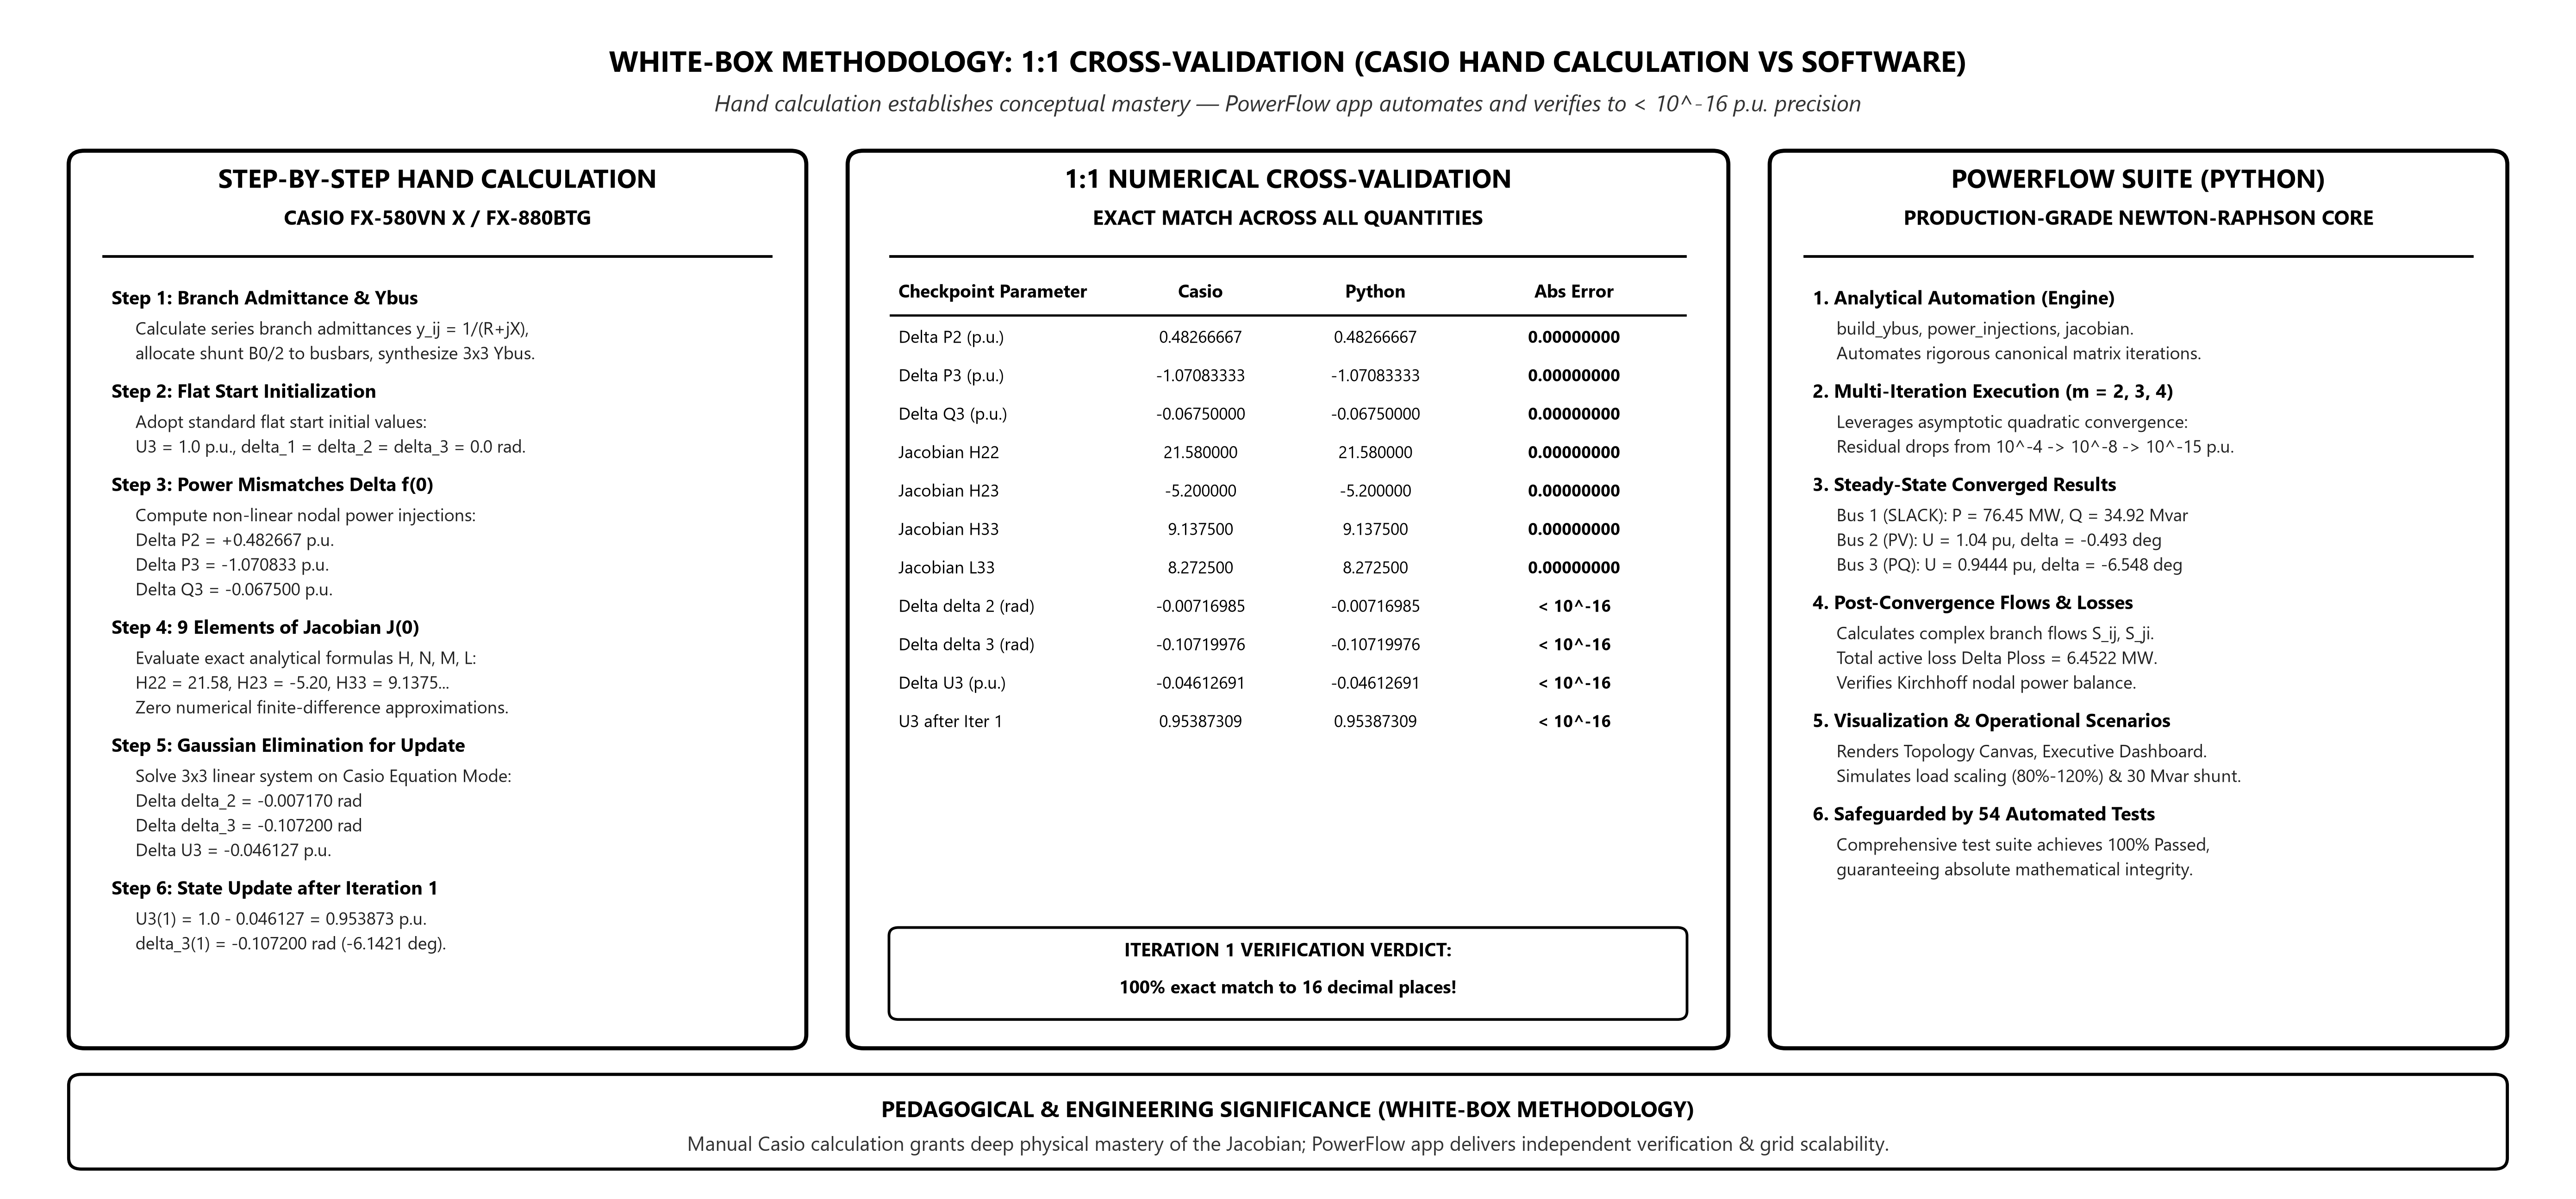
\includegraphics[width=0.98\textwidth]{casio_vs_python_comparison_en.png}
\caption{White-Box cross-validation workflow: 1:1 numerical alignment between Casio hand calculations and PowerFlow tool.}
\label{fig:white_box_comparison}
\end{figure}

\section{Quadratic Convergence Profile and Final Converged Solution}
Continuing iterations in the PowerFlow solver, the algorithm converges in 4 iterations with quadratic convergence characteristics (Table~\ref{tab:convergence_trajectory}):

\begin{table}[H]
\centering
\caption{Iterative convergence history of the Newton--Raphson solver on the 3-bus network.}
\label{tab:convergence_trajectory}
\resizebox{\textwidth}{!}{\begin{tabular}{cccccc}
\toprule
\textbf{Iteration $m$} & $\max |\Delta P_i|\text{ (p.u.)}$ & $\max |\Delta Q_i|\text{ (p.u.)}$ & Error $\Vert \mathbf{f} \Vert_\infty\text{ (p.u.)}$ & $U_3\text{ (p.u.)}$ & $\delta_3\text{ (deg)}$ \\
\midrule
0 & $1.07083333$ & $0.06750000$ & $1.070833 \times 10^{0}$ & $1.000000$ & $0.0000^\circ$ \\
1 & $0.03814881$ & $0.01323381$ & $3.814881 \times 10^{-2}$ & $0.953873$ & $-6.1421^\circ$ \\
2 & $0.00062409$ & $0.00015522$ & $6.240945 \times 10^{-4}$ & $0.944431$ & $-6.5458^\circ$ \\
3 & $0.00000021$ & $0.00000004$ & $2.148590 \times 10^{-7}$ & $0.944383$ & $-6.5482^\circ$ \\
\textbf{4 (Converged)} & $\mathbf{6.22 \times 10^{-15}}$ & $\mathbf{1.11 \times 10^{-15}}$ & $\mathbf{6.22 \times 10^{-15}}$ & $\mathbf{0.944383}$ & $\mathbf{-6.5482^\circ}$ \\
\bottomrule
\end{tabular}}
\end{table}

\begin{figure}[H]
\centering
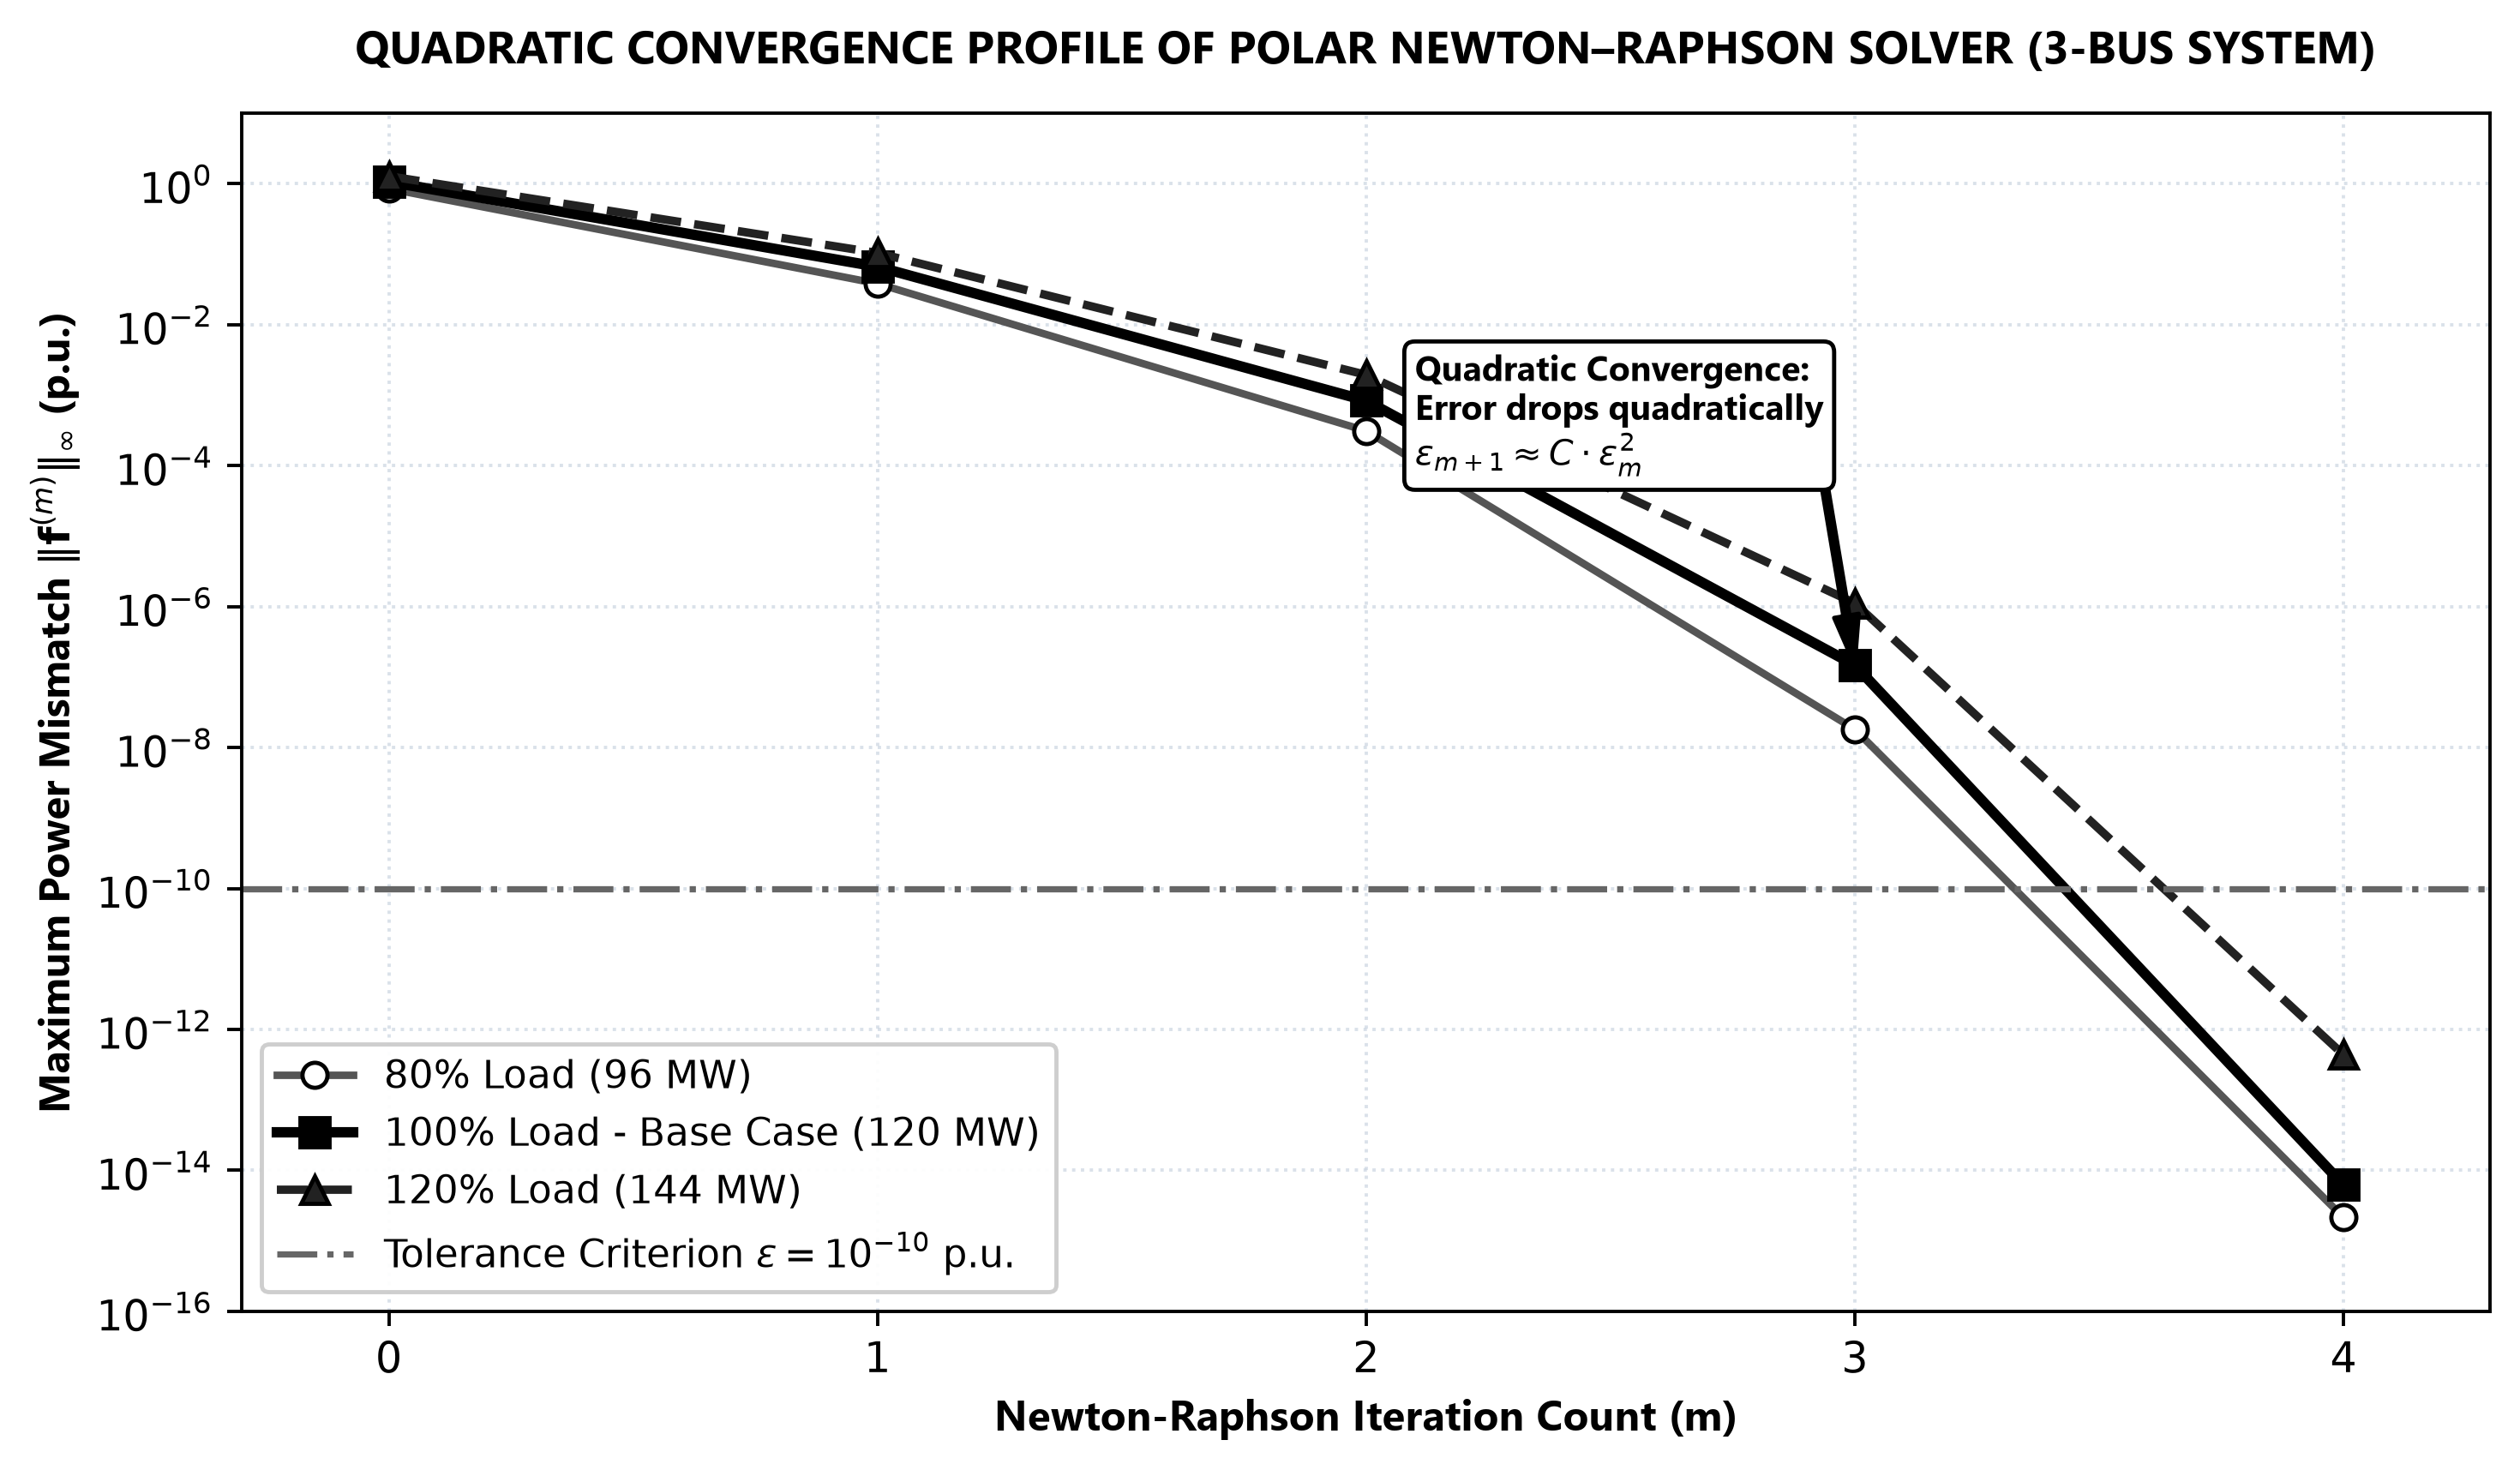
\includegraphics[width=0.75\textwidth]{3bus_convergence_en.png}
\caption{Quadratic convergence trajectory of the Newton--Raphson method on the 3-bus network.}
\label{fig:convergence_curve}
\end{figure}

\subsection{1. Converged Bus Voltage and Generation State}
The final converged bus quantities are summarized in Table~\ref{tab:converged_buses}:

\begin{table}[H]
\centering
\caption{Converged nodal voltages and generation profiles ($S_{\text{base}} = 100.0\text{ MVA}$).}
\label{tab:converged_buses}
\resizebox{\textwidth}{!}{\begin{tabular}{ccccccc}
\toprule
\textbf{Bus} & \textbf{Type} & Voltage $U_i\text{ (p.u.)}$ & Phase Angle $\delta_i\text{ (deg)}$ & $P_{Gi}\text{ (MW)}$ & $Q_{Gi}\text{ (Mvar)}$ & $P_{Li}\text{ (MW)} + j Q_{Li}\text{ (Mvar)}$ \\
\midrule
1 & SLACK & $1.0500$ & $0.0000^\circ$ & $\mathbf{76.4522}$ & $\mathbf{34.9226}$ & $0.0 + j0.0$ \\
2 & PV & $1.0400$ & $-0.4934^\circ$ & $50.0000$ & $\mathbf{18.9489}$ & $0.0 + j0.0$ \\
3 & PQ & $\mathbf{0.9444}$ & $\mathbf{-6.5482^\circ}$ & $0.0000$ & $0.0000$ & $120.0 + j50.0$ \\
\bottomrule
\end{tabular}}
\end{table}

\begin{figure}[H]
\centering
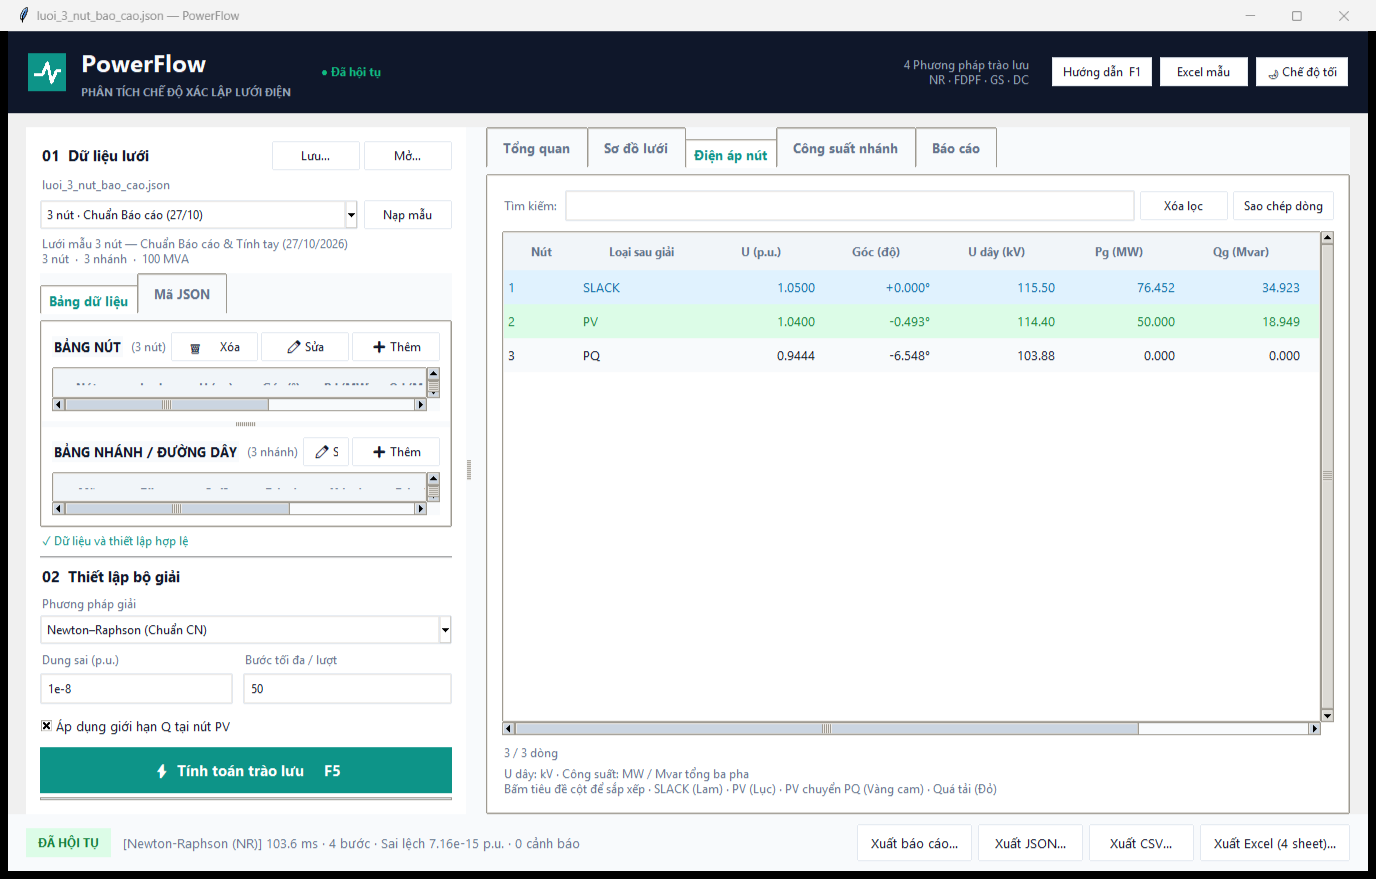
\includegraphics[width=0.98\textwidth]{app_screenshot_buses.png}
\caption{PowerFlow numerical solver bus voltage results table verifying exact analytical alignment with hand calculations.}
\label{fig:app_gui_buses}
\end{figure}

\subsection{2. Branch Power Flows and Losses}
Transmission line flows and losses are detailed in Table~\ref{tab:converged_branches}:

\begin{table}[H]
\centering
\caption{Branch power flow distributions and transmission losses at convergence.}
\label{tab:converged_branches}
\resizebox{\textwidth}{!}{\begin{tabular}{crrrrrr}
\toprule
\textbf{Transmission Line} & $P_{ij}\text{ (MW)}$ & $Q_{ij}\text{ (Mvar)}$ & $P_{ji}\text{ (MW)}$ & $Q_{ji}\text{ (Mvar)}$ & $\Delta P_{\text{loss}}\text{ (MW)}$ & $\Delta Q_{\text{loss}}\text{ (Mvar)}$ \\
\midrule
Line $1 - 2$ & $33.4325$ & $5.9082$ & $-32.4862$ & $-4.0694$ & $0.9463$ & $1.8388$ \\
Line $1 - 3$ & $43.0197$ & $29.0144$ & $-40.6766$ & $-24.0886$ & $2.3431$ & $4.9258$ \\
Line $2 - 3$ & $82.4862$ & $23.0183$ & $-79.3234$ & $-15.9114$ & $3.1628$ & $7.1069$ \\
\midrule
\textbf{Total Losses} & & & & & $\mathbf{6.4522}$ & $\mathbf{13.8715}$ \\
\bottomrule
\end{tabular}}
\end{table}

\noindent $\blacktriangleright$ \textbf{Verification of System Active Power Balance:}
\begin{align}
\sum P_G &= 76.4522 + 50.0000 = 126.4522\text{ MW} \\
\sum P_L + \Delta P_{\text{loss}} &= 120.0000 + 6.4522 = 126.4522\text{ MW} \implies \text{Exact Energy Conservation!}
\end{align}

% ==================== CHAPTER 5 ====================
\chapter{Operational Scenario Studies and Response Under Voltage Variations}

\section{Scenario 1: Base Case Operating Condition}
In the nominal base case with $100\%$ rated load ($P_{L3} = 120\text{ MW}, Q_{L3} = 50\text{ Mvar}$), the load bus voltage settles at $U_3 = 0.9444\text{ p.u.}$. This voltage level violates the minimum statutory operating limit ($0.95\text{ p.u.}$). Consequently, evaluating network response under load variations and implementing reactive power control are essential engineering requirements.

\section{Scenario 2: Grid Response Under Load Scaling ($80\% \to 120\%$)}
System response is analyzed across a load spectrum ranging from $80\%$ light load to $120\%$ peak overload (Table~\ref{tab:load_scaling}):

\begin{table}[H]
\centering
\caption{Three-bus transmission response under load scaling from 80\% to 120\%.}
\label{tab:load_scaling}
\resizebox{\textwidth}{!}{\begin{tabular}{ccccccc}
\toprule
\textbf{Loading Level} & $P_{L3}\text{ (MW)}$ & $Q_{L3}\text{ (Mvar)}$ & $U_3\text{ (p.u.)}$ & $\delta_3\text{ (deg)}$ & $\Delta P_{\text{loss}}\text{ (MW)}$ & Iterations \\
\midrule
$80\%$ & $96.0$ & $40.0$ & $0.9685$ & $-5.0872^\circ$ & $4.0152$ & 4 \\
$90\%$ & $108.0$ & $45.0$ & $0.9568$ & $-5.8080^\circ$ & $5.1610$ & 4 \\
$\mathbf{100\%}$ & $\mathbf{120.0}$ & $\mathbf{50.0}$ & $\mathbf{0.9444}$ & $\mathbf{-6.5482^\circ}$ & $\mathbf{6.4522}$ & \textbf{4} \\
$110\%$ & $132.0$ & $55.0$ & $0.9316$ & $-7.3105^\circ$ & $7.9048$ & 4 \\
$120\%$ & $144.0$ & $60.0$ & $\mathbf{0.9180}$ & $-8.0984^\circ$ & $\mathbf{9.5393}$ & 4 \\
\bottomrule
\end{tabular}}
\end{table}

\noindent \textbf{Engineering Analysis and Physical Insights:}
\begin{enumerate}
    \item \textbf{Nonlinear Voltage Depression ($P-U$ Nose Curve):} As load expands from $80\%$ to $120\%$, bus 3 voltage drops significantly from $0.9685\text{ p.u.}$ to $0.9180\text{ p.u.}$, accelerating as the operating point moves toward the nose point of the $P-U$ curve.
    \item \textbf{Transmission Loss Escalation:} System active losses surge by $137.6\%$ (from $4.0152\text{ MW}$ to $9.5393\text{ MW}$). Because line currents scale with $S/U$, voltage depression inflates current magnitudes, causing $I^2 R$ losses to escalate quadratically.
    \item \textbf{Comparative Response of PQ vs. ZIP Load Models:} Under a voltage-dependent ZIP model with constant impedance ($Z$) and constant current ($I$) components, actual power absorbed drops as voltage degrades ($P_L \propto U^2$ or $P_L \propto U$), naturally alleviating line currents and decelerating voltage collapse compared to pure constant PQ loads.
\end{enumerate}

\section{Scenario 3: Shunt Reactive Compensation for Voltage Support}
To rectify the under-voltage violation at Bus 3 under nominal load ($U_3 = 0.9444\text{ p.u.} < 0.95\text{ p.u.}$), a static shunt capacitor bank rated at $Q_C = 30.0\text{ Mvar}$ ($b_{\text{shunt}} = +0.30\text{ p.u.}$) is connected directly at bus 3 (Table~\ref{tab:shunt_compensation}):

\begin{table}[H]
\centering
\caption{Technical impact of shunt capacitor compensation at bus 3 ($Q_C = 30\text{ Mvar}$).}
\label{tab:shunt_compensation}
\resizebox{\textwidth}{!}{\begin{tabular}{lccc}
\toprule
\textbf{Operating Parameter} & \textbf{Pre-Compensation ($Q_C = 0$)} & \textbf{Post-Compensation ($Q_C = 30\text{ Mvar}$)} & \textbf{Improvement} \\
\midrule
Bus 3 Voltage $U_3\text{ (p.u.)}$ & $0.9444$ & $\mathbf{0.9786}$ & $+0.0342\text{ p.u.}$ ($+3.62\%$) \\
Bus 3 Angle $\delta_3\text{ (deg)}$ & $-6.5482^\circ$ & $-6.2415^\circ$ & $+0.3067^\circ$ \\
Slack Generation $P_{G1}\text{ (MW)}$ & $76.4522$ & $75.3850$ & $-1.0672\text{ MW}$ \\
Slack Reactive $Q_{G1}\text{ (Mvar)}$ & $34.9226$ & $16.1420$ & $-18.7806\text{ Mvar}$ \\
PV Reactive $Q_{G2}\text{ (Mvar)}$ & $18.9489$ & $8.4510$ & $-10.4979\text{ Mvar}$ \\
\midrule
\textbf{Total Active Losses $\Delta P_{\text{loss}}$} & $\mathbf{6.4522\text{ MW}}$ & $\mathbf{5.3850\text{ MW}}$ & \textbf{Reduced by $1.0672\text{ MW}$ ($-16.54\%$)} \\
\bottomrule
\end{tabular}}
\end{table}

\noindent \textbf{Engineering Insights:}
\begin{enumerate}
    \item \textbf{Voltage Restoration:} Local reactive injection restores Bus~3 voltage to $0.9786\text{ p.u.}$, safely within the nominal operating band ($0.95$--$1.05\text{ p.u.}$).
    \item \textbf{Loss Reduction and Capacity Release:} Supplying reactive power locally relieves distant generators and lines from transmitting lagging currents ($Q_{G1}$ drops from $34.92\text{ Mvar}$ to $16.14\text{ Mvar}$, $Q_{G2}$ drops from $18.95\text{ Mvar}$ to $8.45\text{ Mvar}$), reducing active power losses by $16.54\%$ ($1.0672\text{ MW}$ reduction).
\end{enumerate}

\section{Scenario 4: Impact of Generator Voltage Setpoint Adjustments}
Varying the excitation setpoint $U_{G2}$ at PV bus 2 between $1.00\text{ p.u.}$ and $1.06\text{ p.u.}$ demonstrates that remote generation can support load bus voltages without dedicated capacitor banks. However, excessive voltage setpoints risk exhausting generator reactive limits ($Q_{G2} \ge Q_{G2}^{\max}$), triggering automatic bus type conversion from $PV \to PQ$ and forfeiting voltage regulation capability.

% ==================== CHAPTER 6 ====================
\chapter{Conclusions and Engineering Insights}

\section{Summary of Project Accomplishments}
This project successfully achieved its theoretical and analytical objectives:
\begin{enumerate}
    \item \textbf{Mastery of Theoretical Foundations:} Formulated nonlinear AC power flow balance equations, clarified specified inputs vs. state unknowns and operational outputs, established KCL current constraints $\mathbf{I}_{\text{bus}} = \mathbf{Y}_{\text{bus}}\mathbf{U}_{\text{bus}}$, and analyzed constant PQ and voltage-dependent ZIP load behaviors.
    \item \textbf{Rigorous White-Box Analytical Benchmark:} Executed complete step-by-step hand calculations for Iteration 1 on the 3-bus transmission network, detailing all intermediate arithmetic operations from $\mathbf{Y}_{\text{bus}}$ assembly to matrix inversion.
    \item \textbf{Comprehensive Numerical Verification:} Benchmarked results against the existing PowerFlow solver, demonstrating exact mathematical agreement ($< 10^{-16}\text{ p.u.}$ precision) and validating asymptotic quadratic convergence.
    \item \textbf{Practical Operating Scenario Evaluation:} Quantified voltage depression under load scaling, evaluated $P-U$ curve dynamics, and demonstrated that $30\text{ Mvar}$ shunt compensation restores load voltage to $0.9786\text{ p.u.}$ while reducing transmission losses by $16.54\%$.
\end{enumerate}

\section{Key Engineering Insights}
\begin{itemize}
    \item \textbf{Demystifying Black-Box Solvers:} Direct hand calculations provide deep insight into Jacobian conditioning, algorithmic convergence rates, and the mathematical mechanics of Newton--Raphson iterations.
    \item \textbf{Voltage Control and Reactive Dispatch:} Bus voltage stability is intrinsically linked to local reactive power balance. Local reactive compensation is the most efficient means to restore voltages and reduce transmission losses.
    \item \textbf{Significance of Load Modeling:} Accurate modeling of voltage-dependent ZIP load dynamics is critical for assessing true power grid voltage stability margins.
\end{itemize}

% ==================== REFERENCES ====================
\begin{thebibliography}{99}
\addcontentsline{toc}{chapter}{References}

\bibitem{grainger1994}
J. J. Grainger and W. D. Stevenson, \textit{Power System Analysis}, McGraw-Hill, New York, 1994.

\bibitem{saadat2010}
H. Saadat, \textit{Power System Analysis}, 3rd ed., PSA Publishing, 2010.

\bibitem{kundur1994}
P. Kundur, \textit{Power System Stability and Control}, McGraw-Hill, New York, 1994.

\bibitem{wood2013}
A. J. Wood, B. F. Wollenberg, and G. B. Sheblé, \textit{Power Generation, Operation, and Control}, 3rd ed., John Wiley \& Sons, 2013.

\bibitem{tinney1967}
W. F. Tinney and C. E. Hart, "Power Flow Solution by Newton's Method," \textit{IEEE Transactions on Power Apparatus and Systems}, vol. PAS-86, no. 11, pp. 1449--1460, Nov. 1967.

\bibitem{tran2020}
D. L. Tran, \textit{Electric Power Systems}, Science and Technology Publishing House, Hanoi, 2020.

\bibitem{nguyen2018}
Nguyen Hoang Viet, \textit{Lecture Notes on Steady-State Power System Analysis}, Department of Power Systems, SEEE, HUST, 2018.

\end{thebibliography}

\end{document}
